\section{운영체제 병렬화 역사}
본 장에서는 그 동안 많이 연구되어온 운영체제 병렬화가 현시점에서 필요한 이유와 함께 
운영체제의 병렬화 역사에 관해서 설명한다.
그 동안 운영체제의 병렬화는 시분활 시스템, 클라이언트(Client) 서버(Server) 구조, 그리고 SMPs(Shared Memory
Processor) 그리고 최근 프로세서에 코어가 많아 지는 멀티코어로 총 4단계로 발전해 왔다~\cite{Kaashoek2015PCO}.

첫 번째 단계에서는 시분활 시스템에서 사용되는 운영체제 병렬화이다. 
60년대부터 70년대의 운영체제 병렬성에 대한 연구는 시분할(Time Sharing) 시스템을 대상으로 하였다.
즉 컴퓨터 한대에 여러 사용자가 동시에 사용되기 시작하였으나 대부분 시스템은 1개의 프로세서로 이루어졌다.
따라서 이 시점에서 병렬 처리 연구는 I/O 병렬화 프로그램에 대한 연구가 많이 진행되었다~\cite{Bloch1959EDS}.
즉 최대한 프로세서를 이용률(Utilization)를 높임과 동시에 I/O를 병렬로 처리하기 위한 방법들이 연구되었다.
따라서 이 당시 커널은 병렬로 I/O를 처리하기 위해 다른 프로그램 커널로 문맥교환되어 실행되도록 만들어졌다.
 
초기 컴퓨터 중 일부 프로세서들은 시분활 시스템과 멀티프로세서의 병렬화를 고려하여 
만들었다(예를 들어, 버로우스(Burroughs)의 B5000~\cite{Mayer1982ABB}).
따라서, 병렬화에 대해서 많은 관심과 노력이 이루어졌다.
그 결과 병렬화 관련 초기 많은 이론인 암달의 법칙~\cite{Amdahl1967VSP}, 멀틱스(Multics)에서의 트래픽 컨트롤
~\cite{Saltzer1966TCM}, 데드락 디텍션(Deadlock Detection) 그리고 락 오더링(Locking
Ordering)등 많은 이론들이 이 당시 생겨나게 되었다. 
70년대 하나의 프로세서 위에서 병렬화를 제공하기 위해 많은 연구 및 개발이 이루어졌고, 
리눅스 커널의 조상인 단일 프로세스에 여러 유저에게 시분활 기능으로 병렬화를 제공하는 
Unix 커널~\cite{Ritchie1973UTS}이 이 당시 개발되었다.

두 번째 단계에서는 80년대와 90년대에는 컴퓨터의 가격이 개인이 구매가 가능할 정도 내려갔으며, 
로컬 네트워크로 여러 유저가 협업하면서 작업할 수 있는 환경이 되면서 클라인트 서버 환경을 위한 
병렬화가 연구가 이루어졌다.
이 당시 문제는 여러 유저가 수행할 서비스(Services)에 대한 병렬화가 필요하게 되었고, 
따라서 응용 프로그래머들도 커널의 기능이 필요하게 되었으며, 
이를 위해 서버의 커널에 인터페이스(Interface)를 추가하여 동시에 여러 유저들에게 
병렬화된 서비스를 제공하였다. 
 
그 결과 많은 운영체제 병렬화 기술들이 이 시점에 연구 개발되었다. 
예를 들어 스레드(Thread), 락(Locks) 그리고 컨디션 변수(Condition Variables)등 이 시점에 많은 연구가 이루어졌다.
이벤트(events)와 스레드(threads)에 대한 논쟁~\cite{Ous96}~\cite{vonBehren2003WEB} 그리고
Accent~\cite{Rashid1981ACO}, Mach~\cite{Accetta86mach} , V~\cite{Cheriton1983DVK} 등 새로운 
운영체제들이 제안되었다. 
이러한 연구들은 결국 마이크로커널(Microkernel)에 영감을 주었고, 결국 최근 많은 운영체제가 사용하고 있는 
Pthreads[POSIX.1c, Threads extensions (IEEE Std 1003.1c-1995)]에게도 많은 영향을 주었다. 
이 당시 새로운 운영체제 뿐만 아니라 새로운 언어들(예를들어 Mesa~\cite{Lampson1979EPM})도 
연구되었고, 결국 가비지 컬렉션등에 대한 연구가 이 순간 진행되었으며, 그 결과 
최근 자바(JAVA)와 고(Go) 언어등 가비지 컬랙션(Garbage Collection) 기반 언어에많은 영감을 주었다.
결론으로 이 시점의 연구들은 커널의 인터페이스를 서버 개발자에게 노출하여 서버를 
병렬로 이용 할 수 있게 만들었다.

\begin{figure}[h!]
    \centering
    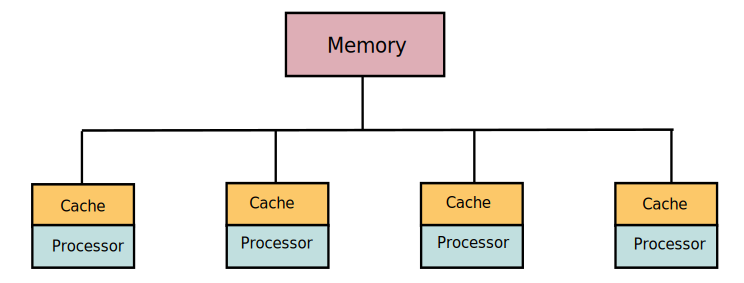
\includegraphics[width=0.8\textwidth]{fig/shared_memory}
    \caption{90년대 공유 메모리 시스템}
  \label{shared_memory}
\end{figure}

다음 단계에서는 90년대 각각의 프로세서가 메모리를 공유하는 개념의 컴퓨터인 SMP(Shared-memory Multi
Pocessors)가 낮은 가격으로 보급이 되어서, 커널 또는 서버 개발자는 이 당시부터 심각하게 
운영체제 병렬화에 대해서 고려하게 되었다.
예를 들어, 리눅스 커널은 BKL(Big Kernel Lock) 등을 이 당시부터 지원하며 병렬화 기능을 제공하기 시작하였다.
이 시점 많은 회사(BBN Butterfly, Sequent, SGI, Sun, Thinking Machines 등)도 역시 운영체제 병렬화에
대해서 연구하기 시작했다.
그 결과 많은 운영체제 성능 확장성에 대해서 새로운 개념(예를들어, 
MCS 락~\cite{MellorCrummey1991MCS}, 유저 레벨 스레딩~\cite{Marsh1991FUT}, NUMA 메모리
관리~\cite{Bolosky1991NPR}, 가상 머신 모니터(Virtual Machines
Monitor)~\cite{Bugnion1997DRC})들이 제안되었다.  

\begin{figure}[h!]
  \begin{center}
    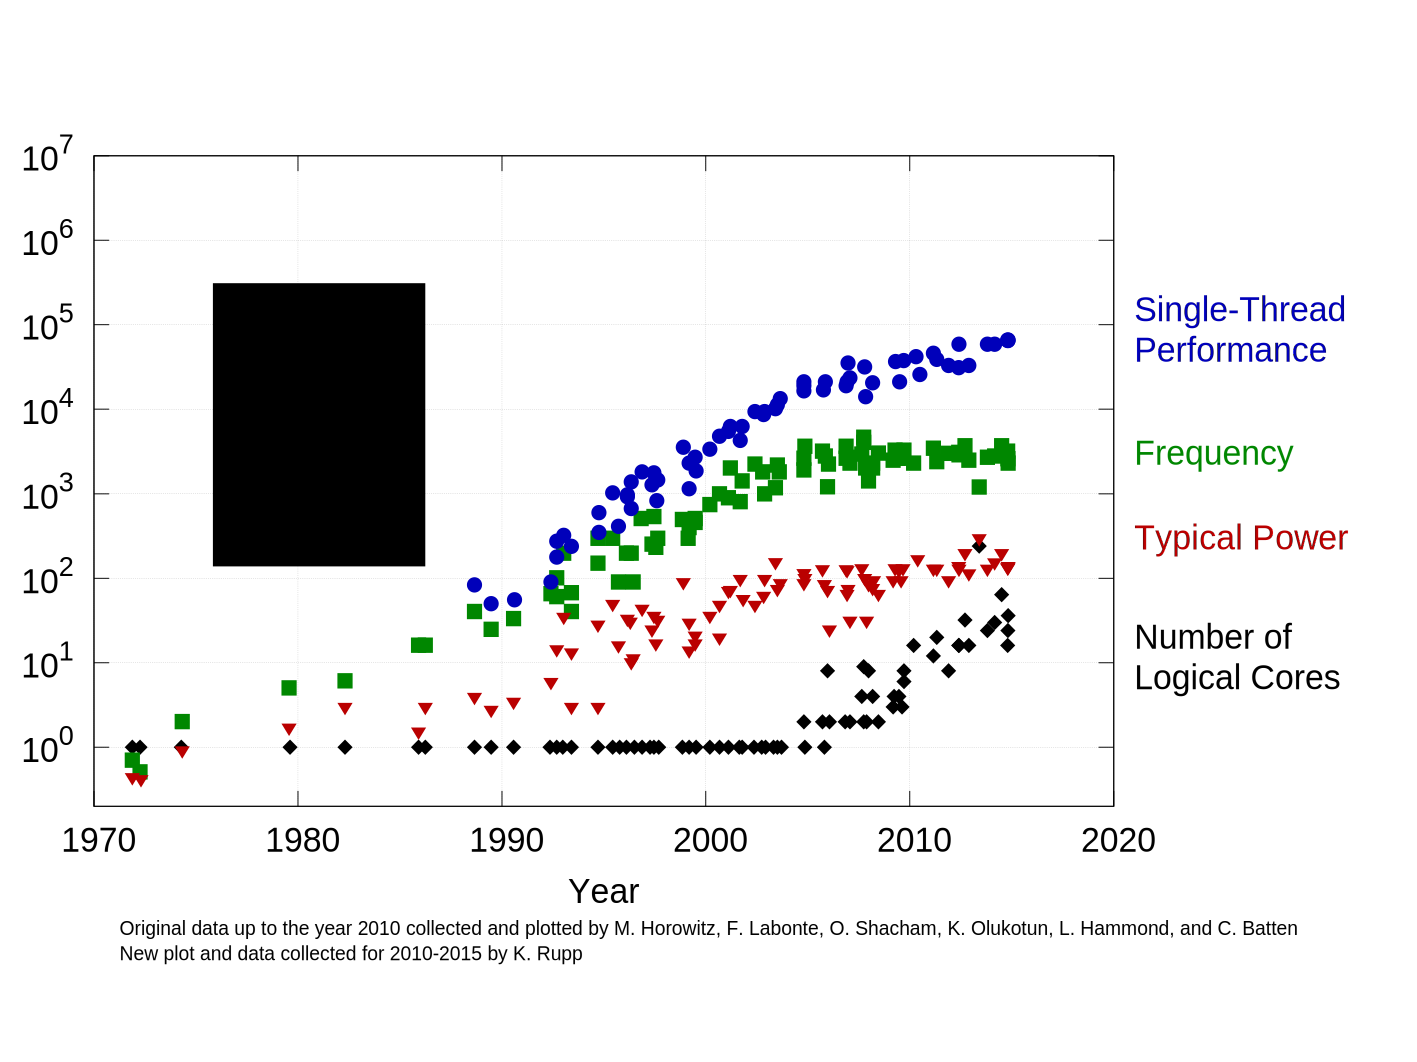
\includegraphics[scale=0.3]{fig/cpu}
  \end{center}
  \caption{CPU 발전 동향.}
  \label{fig:aim7}
\end{figure}

마지막 단계는 멀티코어 단계이다.
그림~\ref{fig:aim7}과 같이 주파수는 계속 증가하다가, 2000년대 중반 멈추고, 그 때부터 코어 수가 증가하고 있다. 
따라서 코어수가 100개 이상의 멀티코어 프로세서들도 등장함에 따라, 이 때 부터 멀티코어 공유 
메모리 시스템 때문에 야기하는 새로운 문제가 발생하기 시작하였다.

\begin{figure}[h!]
    \centering
    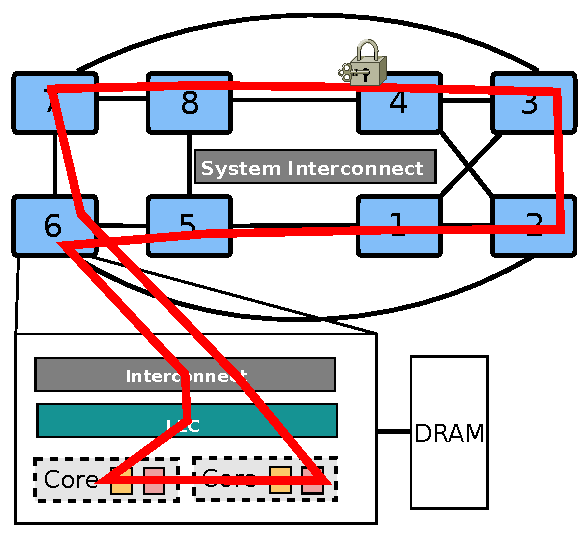
\includegraphics[width=0.6\textwidth]{fig/archcache}
    \caption{공유 메모리 시스템}
  \label{shared_memory}
\end{figure}

이러한 새로운 문제들은 상당 부분이 캐시라인(Cache-line)의 공유 때문에 발생하는 문제이다.
그림~\ref{shared_memory}은 이러한 문제를 보여준다. 
그 이유는 시스템에 인터커넥트(Interconnect)는 하나이며, 이것이 결국 병목이 된다. 
그림에서 4번 NUMA 노드의 코어가 데이터를 변경하면, 그것을 읽고 있는 코어들이 
모두 시스템 인터커넥트로 캐시 일관성 프로토콜 메시지를 전송하게 되어 결국 시스템 인터커넥트는 
굉장히 바뻐지게 된다. 
이로 인해 코어가 증가 할 수록 한개로 구성되어 있는 인터커넥트로 인해 확장성이 떨어지게 되는 문제가 있다. 
따라서, 이러한 문제를 해결하기 위해서 많은 연구들이 진행되고 있다. 

\begin{figure}[h!]
    \centering
    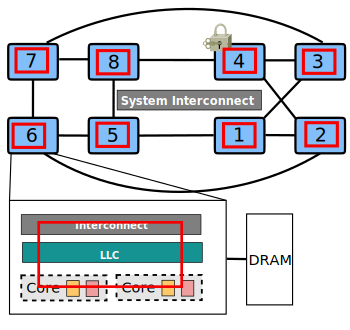
\includegraphics[width=0.6\textwidth]{fig/archcache_percore}
    \caption{공유 메모리 시스템}
  \label{shared_memory2}
\end{figure}

이처럼 멀티코어를 대상으로 병렬화가 연구가 되다가, 최근에는 매니코어에서 발생하는 
캐시 일관성 트래픽 문제를 해결하기 위해 여러 파티션닝 기법들이 연구되고 있다.  
파티션닝 기법 중 가장 쉽게 생각할 수 있는 방법은 공유 메모리의 자료 구조를 각자 
CPU에서 처리하도록 하는 즉 퍼코어 구조의 알고리즘을 사용하는 방법이 있다.
퍼코어 구조의 방법은 그림~\ref{shared_memory2}와 같이 메모리에 데이터가 수정되어도 시스템 
인터커넥트에 캐시 일관성 프로토콜 메시지를 전송하지 않으므로, 
시스템 전반에 발생하는 캐시 커뮤니케이션 오버헤드를 줄일 수 있다. 

이번 장은 최신에 발생하는 확장성 문제를 해결하기 위해, 확장성 있는
운영체제(section~\ref{sec:osrelated}), 확장성 있는 락(section~\ref{sec:lockrelated}), 
그리고 확장성 있는 자료구조와 알고리즘(section~\ref{sec:datarelated})들이 어떻게 연구되고 
있는지를 설명한다.

%$$$$$$$$$$$$$$$$$$$$$$$$$$$$$$$$$$$$$$$$$$$$$$$$$$$$$$$$$$$$$$$$$$$$$$$$$$$$$$$$
%Paragraph 1:Linux Scalability의 연구에 대한 설명
%$$$$$$$$$$$$$$$$$$$$$$$$$$$$$$$$$$$$$$$$$$$$$$$$$$$$$$$$$$$$$$$$$$$$$$$$$$$$$$$$

\newpage
\section{최근 운영체제 병렬화 연구}
\label{sec:osrelated}

%~\cite{Boyd-WickizerCorey}~\cite{Wentzlaff2010fOS}
%~\cite{Baumann2009Barrelfish}
%~\cite{Liu2009Tessellation}~\cite{Farrington2010Helios}

최근 병렬화 운영체제에 대한 연구는 새로운 확장성 있는 운영 체제를 만들거나 
기존 운영체제를 최적화 시키는 방향으로 연구가 진행되고 있다.
%~\cite{SilasBoydWickizer2010LinuxScales48}
%~\cite{AustinTClements2012RCUBalancedTrees}~\cite{Clements2013RadixVM}~\cite{SilasBoydWickizerPth}


\subsection{새로운 운영체제 제안}

\subsubsection{Corey}
Corey~\cite{Boyd-WickizerCorey}는 MIT의 PDOS(Parallel and Distributed Operating
Systems)에서 개발하였다.
Corey의 기본 철학은 커널 영역의 공유 데이터를 유저 응용프로그램이 사용할 수 있도록 인터페이스를 제공 함에 따라,
공유 데이터 때문에 발생하는 경합 문제를 유저 응용프로그램이 해결할 수 있도록 하는 것이다.
Corey가 이러한 방법을 사용한 이유는 매니코어 시스템에서는 코어 간의 캐시 일관성 작업 
때문에 성능이 저하되고, 이 현상이 발생하는 근본 원인이 운영체제가 응용프로그램의 특성에 관계 없이 
불필요하게 데이터를 공유하기 때문이다.
또한 하드웨어 역시 응용프로그램의 특성에 상관없이 캐시 메모리를 동기화 하는 방식을 사용하기 때문에,
기존 운영체제에서 취하는 방법을 사용하면 공유 문제를 해결 할 수 없다는 것이다.  
즉 기존 해결 방법들은 매니코어 환경에서 응용프로그램 특성에 따라 최적화 할 수 없다는 문제점을 가진다. 
이러한 문제를 해결하기 위해, Corey는 응용프로그램의 워크로드에 따라 공유 문제를 응용프로그램 작성자가 
직접 해결할 수 있는 방법을 제공해준다.
이러한 방법은 과거 연구되어온 커널의 자원을 유저와 공유할 수 있는 Exokernel~\cite{Engler1995EOS}의 개념을 가져와 
매니코어 시스템에 적용한 방법이며, Corey는 Exokernel의 개념을 통해 확장성을 개선하였다.


\begin{figure}[h!]
    \centering
    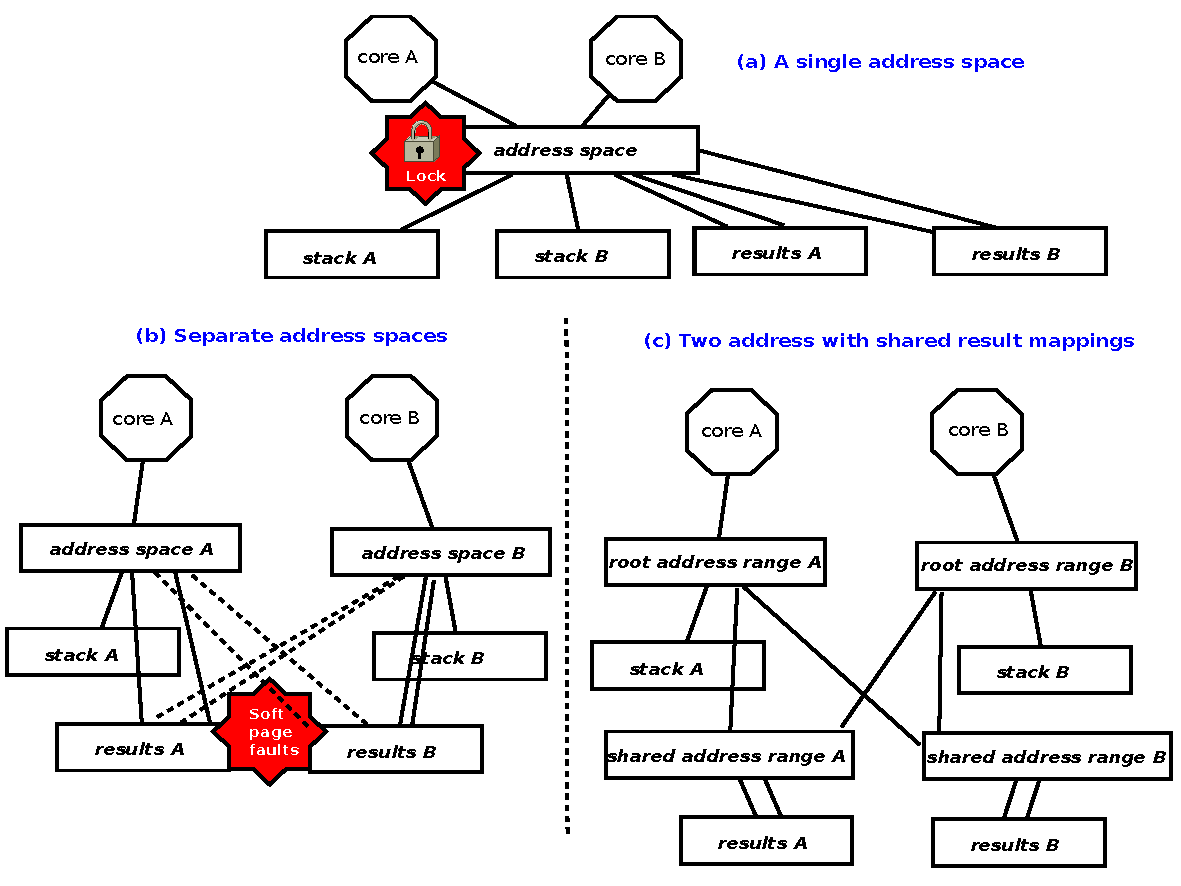
\includegraphics[width=1\textwidth]{fig/corey/corey}
    \caption{corey 운영체제 address space 공유 방법}
  \label{fig:corey}
\end{figure}

%$$$$$$$$$$$$$$$$$$$$$$$$$$$$$$$$$$$$$$$$$$$$$$$$$$$$$$$$$$$$$$$$$$$$$$$$$$$$$$$$
%Paragraph 2:Corey의 3가지 기본 개념 설명
%$$$$$$$$$$$$$$$$$$$$$$$$$$$$$$$$$$$$$$$$$$$$$$$$$$$$$$$$$$$$$$$$$$$$$$$$$$$$$$$$
Corey는 3가지 기본적인 개념(Address Rages, Kernel Core, Shares)을 가지고 있다. 
첫째, Address Rages는 운영체제에서 여러 스레드간의 공유하는 데이터인 Address Space에 대해서 다룬다.
대부분의 운영체제는 Address Space를 그림~\ref{fig:corey}(a)와 같이 Single Address Space로
구성하는 경우 또는 그림~\ref{fig:corey}(b)와 같이 퍼코어 기반의 Separate Address Space로 구성하는 경우로
구성된다. 
만약 Single Address Space를 사용할 경우 모든 코어가 같은 Address Space를 공유함에 따라 반드시 락이
필요하고 이 락 때문에 스레드들이 직렬화된다.
예를 들어, 맵리듀스(MapReduce)와 같은 응용프로그램을 사용할 경우 맵 단계에서 굉장히 많은 락 경합이 발생하게 된다.
반대로, Separate Address Space를 사용할 경우 리듀스 단계에서 공유하지 않은 데이터에 접급함에 따라 
소프트 페이지 폴트(Soft Page Fault)가 많이 발생하는 문제가 발생한다.
Corey는 이러한 문제를 Address Rages라는 새로운 개념으로 해결하였다. 
이것은 그림~\ref{fig:corey}(c)와 같이 Separate Address Space를 제공함과 동시에 중간 결과를 공유할 수 있는
방법인 Single Address Space를 제공함에 따라, 두 장점을 동시에 취한다.
다음으로, Kernel Core는 응용프로그램의 공유 메모리를 사용하지 않고, 특정 코어에 
독점 할당 시켜주고 공유는 IPC로 하도록한 기술이다. 
따라서 스케줄러와 인터럽트에 방해를 받지 않고 캐시 지역성을 높여 성능을 향상 시킨다. 
마지막으로, 공유는 Exokernel과 같이 커널 자료구조를 응용프로그램에게 접근할 수 있는 
기능을 제공해준다.


\subsubsection{Barrelfish}

%$$$$$$$$$$$$$$$$$$$$$$$$$$$$$$$$$$$$$$$$$$$$$$$$$$$$$$$$$$$$$$$$$$$$$$$$$$$$$$$$
%Paragraph : Barrelfish의 특징 설명
%$$$$$$$$$$$$$$$$$$$$$$$$$$$$$$$$$$$$$$$$$$$$$$$$$$$$$$$$$$$$$$$$$$$$$$$$$$$$$$$$
Barrelfish~\cite{Baumann2009Barrelfish}는 취히리의 ETH와 마이크로 소프트(Microsoft)가
공동 연구하여 만든 운영체제이다.
Barrelfish는 멀티커널(Multikernel) 운영체제 중 하나 이고, 기본적인 철학은 공유 메모리 시스템 
기능들을 분산 처리 방식으로 구현하는 것이다.
예를 들어, 운영체제에서 각 코어는 마치 네트워크로 분산 된 시스템으로 가정하고, 서로 다른 코어 간에는 메시지 
패싱을 통해 통신을 하여 성능을 향상 시키는 방법이다. 
이러한 방법을 사용한 이유는 캐시 구조로 된 시스템의 단일화된 인터커넥트가 코어가 증가할 수록 캐시 
일관성 트래픽 문제를 야기 하기 때문에, 메시지 패싱 방법이 하나의 인터커넥트를 이용하는 하드웨어 캐시 일관성 
프로토콜을 사용하는 방법보다 오히려 더 높은 성능을 보이기 때문이다. 

%$$$$$$$$$$$$$$$$$$$$$$$$$$$$$$$$$$$$$$$$$$$$$$$$$$$$$$$$$$$$$$$$$$$$$$$$$$$$$$$$
%Paragraph : Barrelfish의 구조 설명 
%$$$$$$$$$$$$$$$$$$$$$$$$$$$$$$$$$$$$$$$$$$$$$$$$$$$$$$$$$$$$$$$$$$$$$$$$$$$$$$$$
이러한 Barrelfish의 구현은 그림~\ref{fig:Barrelfish}과 같다.
커널 레벨에서는 하드웨어와 밀접한 CPU Driver가 하드웨어 인터페이스를 제공한다.
CPU Driver는 유저 레벨의 모니터(Monitor)와 함께 하나의 운영체제 처럼 동작하며, 
이것은 마치 각 코어에 하나의 운영체제가 동작하는 것 처럼 보이는 멀티커널(Multikernel)의 구조를 따른다.
응용프로그램은 여러 코어를 이용할 수 있는데, 이러한 환경을 제공하기 위해 존재하는 것이 모니터이다. 
모니터는 운영체제의 기본 기능을 제공하기 위해 존재하며, 공유 메모리를 사용하기 
보다는 복제(Replication)와 IPC와 같은 분산 시스템에서 사용하는 방법을 이용한다. 
모니터는 View라는 상태를 가지고 복제를 수행한다. 
이러한 방법 공유 메모리 시스템을 분산 시스템에서 사용하는 방식과 같이 시스템을 구성하여, 
캐시 커뮤니케이션 때문에 발생하는 시스템 인터커넥트의 로드를 줄일 수 있다.

\begin{figure}[h!]
    \centering
    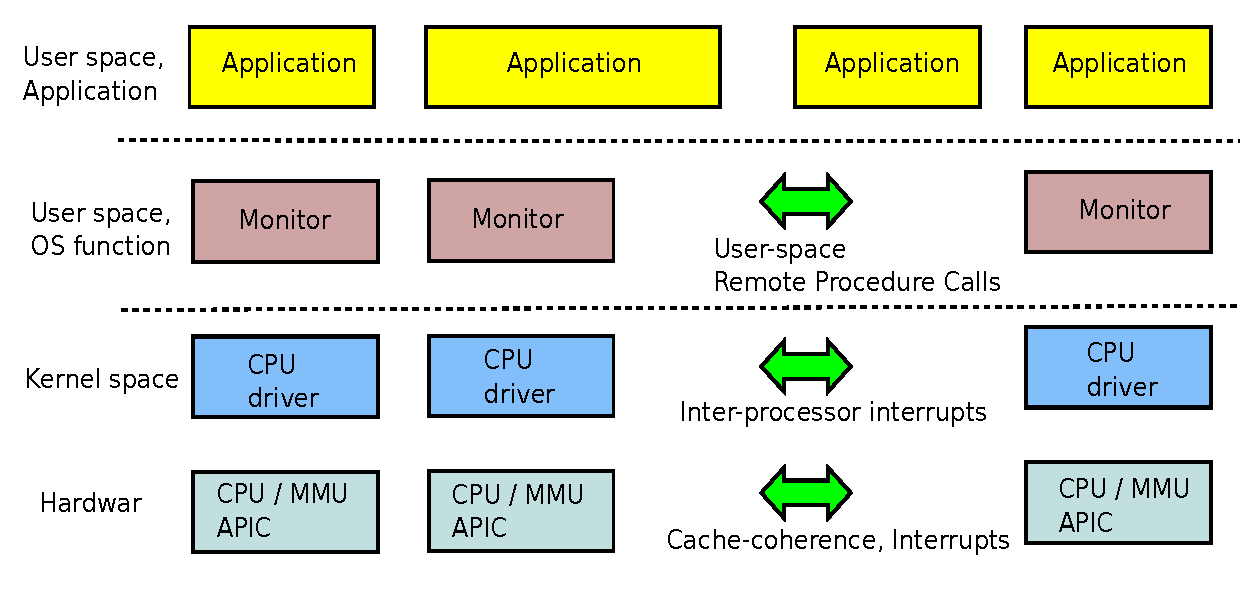
\includegraphics[width=1\textwidth]{fig/multikernel/multikernel}
    \caption{Barrelfish 구조}
  \label{fig:Barrelfish}
\end{figure}

%$$$$$$$$$$$$$$$$$$$$$$$$$$$$$$$$$$$$$$$$$$$$$$$$$$$$$$$$$$$$$$$$$$$$$$$$$$$$$$$$
%Paragraph : Barrelfish의 구조의 단점
%$$$$$$$$$$$$$$$$$$$$$$$$$$$$$$$$$$$$$$$$$$$$$$$$$$$$$$$$$$$$$$$$$$$$$$$$$$$$$$$$
Barrelfish의 단점은 Barrelfish의 구조적인 철학이 공유를 최대한 줄이는 것인데, 
이로 인해 로드 밸런싱을 수행할 수 없는 단점을 가져온다. 
예를 들어 하나의 코어에 여러 스레드들이 같이 돌고 있고, 다른 코어에는 아무런 
스레드도 없는 경우, Barrelfish는 분산 시스템 처럼 수행되므로 동적으로 스레드에 대한 정보들을 
다른 코어로 전송할 수가 없다.
즉 로드 밸런싱이 어려우므로 응용프로그램에 따라,
로드가 한 쪽에 몰리는 경우, 느려진 코어의 스레드들을 기다려야 하기 때문에 전체적인 
성능이 저하된다.  

\subsubsection{FusedOS}
%$$$$$$$$$$$$$$$$$$$$$$$$$$$$$$$$$$$$$$$$$$$$$$$$$$$$$$$$$$$$$$$$$$$$$$$$$$$$$$$$
%Paragraph : Fused OS의 특징 설명
%$$$$$$$$$$$$$$$$$$$$$$$$$$$$$$$$$$$$$$$$$$$$$$$$$$$$$$$$$$$$$$$$$$$$$$$$$$$$$$$$
FusedOS는 IBM 연구소에서 개발되었으며, 모노리틱 구조와 마이크로 구조를 혼합한 운영체제이다.
기존 연구들은 모두 경량 커널(LWK: Light-Weight Kernel) 또는 정량 커널(FWK:
Full-Weight Kernel) 둘 중 하나의 방식으로만 개발되었으나, 이 두가지를 
혼합하여 만든 운영체제이다.
이처럼 혼합하여 만든 운영체제인 FusedOS의 장점은 LWK를 통하여 FWK이 가지고 있는 근본적인 확장성 
문제를 해결함과 동시에, 과학에서 많이 사용되는 특정한 목적으로 개발된 응용프로그램을 
LWK에서 동작시킴에 따라 커널의 간섭이 없이 동작 시킬 수 있다는 것이다. 
또한, FWK의 장점 중 하나인 리눅스로 인하여 기존 만들어진 라이브러리들을 
리눅스의 장점을 모두 활용 할 수 있다.
 
\begin{figure}[h!]
    \centering
    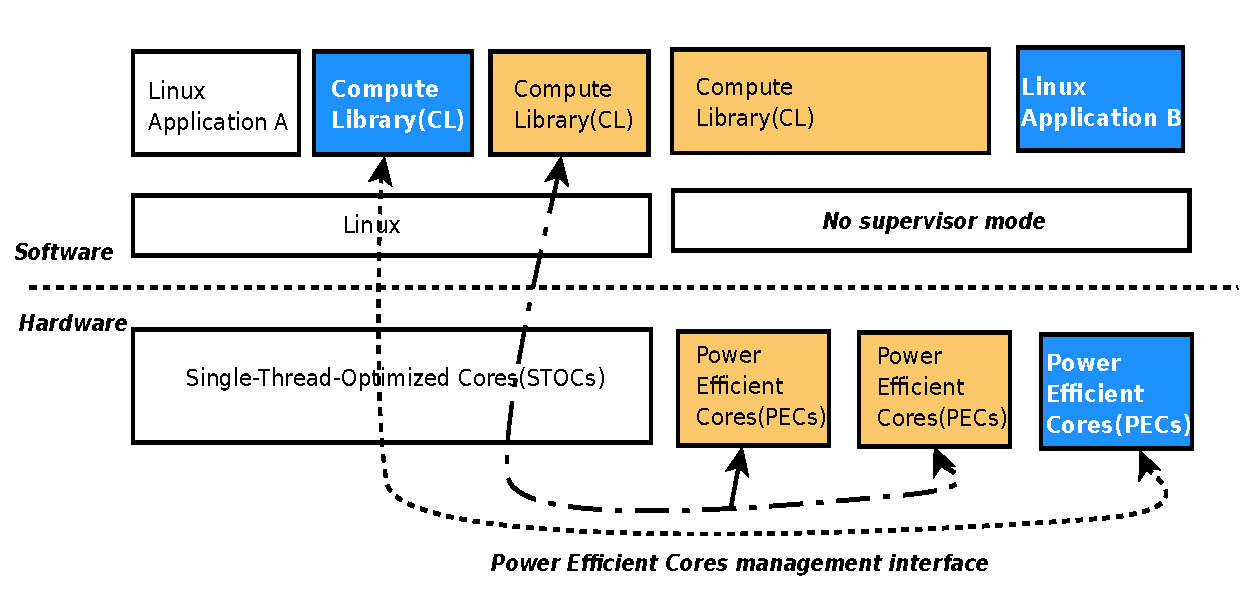
\includegraphics[width=1\textwidth]{fig/fusedos/fusedos}
    \caption{FusedOS 구조}
  \label{fig:FusedOS}
\end{figure}

%$$$$$$$$$$$$$$$$$$$$$$$$$$$$$$$$$$$$$$$$$$$$$$$$$$$$$$$$$$$$$$$$$$$$$$$$$$$$$$$$
%Paragraph : Fused OS의 구조 설명
%$$$$$$$$$$$$$$$$$$$$$$$$$$$$$$$$$$$$$$$$$$$$$$$$$$$$$$$$$$$$$$$$$$$$$$$$$$$$$$$$
이러한 FusedOS의 구조는 그림~\ref{fig:FusedOS}과 같다. 
그림과 같이 FusedOS의 하드웨어는 성능 좋은 코어 그룹(STOCs: Single-Thread-Optimized Cores)과
전력에 효율적인 코어 그룹(PECs: Power Efficient Cores)으로 구성되어 있다.
PEC는 STOC의 기능 중 하나이나 관리자(Supervisor) 모드를 포함하고 있지는 않는다. 
STOC에는 리눅스 운영체제가 동작하고, 기존 리눅스에 기능을 추가하여 Compute Library(CL)이 PEC에 
접근이 가능하도록 설계되었다.

CL은 마치 리눅스 응용프로그램처럼 동작하며, 실행이 되면 다음으로 가벼운 커널을 PEC 커널 쪽 메모리에 
전달하고 그 후 가벼운 커널은 PEC 코어에서 동작하게 된다.
이러한 구조를 통해, HPC 응용의 성능을 보여주면서 리눅스 운영체제의 기능을 제공할 수 있는 장점을 가진다. 
FusedOS의 성능은 HPC 운영체제 코어와 연산을 위한 코어가 분리되었기 때문에, 운영체제의 
방해를 받지 않아 기존 리눅스보다 높은 성능을 보인다.
이것을 통해 기존 운영체제의 병목 현상인 캐시 일관성 유지 때문에 발생하는 확장성 문제를 해결할 수 있다.
하지만 FusedOS의 문제점은 독립적으로 코어에 LWK를 할당하여 호출하는 방법을 사용하므로,  
응용프로그램을 실행하고 종료하는데 추가적인 시간을 가지는 단점이 있다.

\subsection{기존 운영체제 최적화}

\subsubsection{Linux Scalability}

앞에서 설명한 새로운 운영체제에 대한 연구 뿐만 아니라 기존 운영체제의 확장성에 대한 연구가 진행되었다. 
특히 MIT PDOS 연구 그룹은 새로운 운영체제가 아닌 리눅스 커널을 대상으로 매니코어 환경에서 확장성을 연구하였다.
실제 많이 사용되는 7가지의 응용프로그램(Exim, Memcached, Apache, PostgreSQL, Gmake, Psearchy,
MapReduce)을 가지고 MOSBENCH라는 응용프로그램 벤치마크를 만들어 리눅스 커널을 대상으로 실험을 
하였고, 측정 중 발생되는 여러 문제를 해결하여, 종합적인 리눅스 커널의 확장성을 향상시켰다.

\begin{figure}[h!]
    \centering
    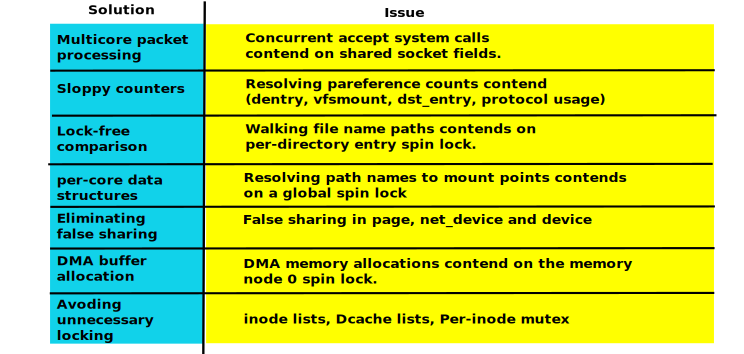
\includegraphics[width=1\textwidth]{fig/linux/linux}
    \caption{linux scalability 분석 연구}
  \label{fig:linux}
\end{figure}

이 연구는 그림~\ref{fig:linux}과 같이 총 7가지의 기술을 활용하였고, 추가적으로 응용프로그램을 직접 수정하여 
커널의 확장성을 개선하였다.
이러한 7가지 기술 중 하나는 멀티코어 패킷 프로세싱이 있다. 
그 동안 리눅스 커널은 네트워크 멀티코어 패킷에 대해서 멀티 큐를 사용하여 성능과 확장성을 이루었으나, 
클라이언트 연결 주기가 짧을 경우 이러한 방법도 여전히 성능과 확장성 문제를 가진다.
따라서 이 연구 그룹은 아파치(Apache) 응용프로그램과 같이 동시 다발 적으로 연결을 요청하는 경우 
퍼코어 큐에 저장하도록 \code{accpet()}을 수정하였다. 
이 것은 싱글 리스닝(Listening) 소켓을 보호하기 위해 존재하는 락을 제거할 수 있으므로 확장성을 향상 시킨다.

다음으로 이 연구 그룹은 리눅스의 참조 카운터 때문에 발생하는 캐시 일관성 트래픽을 제거하기 위해 
\textit{sloppy counter}를 만들었다.
그리고 이 \textit{sloppy counter}를 디렉터리 엔트리 오브젝트(\code{dentrys}), 마운트된 파일 시스템
오브젝트(\code{vfsmounts}) 그리고 네트워크 프로토콜에서의 메모리 할당을 추적하기 위한 전역 변수에 
적용하여 성능 및 확장성을 향상 시켰다.
또한 리눅스 커널은 디렉토리 엔트리 캐시의 이름을 찾는 부분에 \textit{per-dentry spin lock} 때문에 문제가 
있는데, 이 문제를 해결하기 위해 리눅스의 \textit{lock-free page-cache lookup protocol}과
유사한 방법을 만들어 전역 \textit{spin lock}을 제거하였다.
그 이외에도 퍼코어 방법을 사용한 방법과 캐시 라인의 \textit{false sharing} 때문에 발생하는 성능 저하 문제, 
이더넷 디바이스 DMA 버퍼가 한쪽 노드에만 할당되어 발생하는 확장성 문제와 그리고 불필요한 락을 
제거하여 리눅스 커널의 확장성을 향상 시켰다.  

\subsubsection{BonsaiVM}
%$$$$$$$$$$$$$$$$$$$$$$$$$$$$$$$$$$$$$$$$$$$$$$$$$$$$$$$$$$$$$$$$$$$$$$$$$$$$$$$$
%Paragraph : BonsaiVM 특징 설명
%$$$$$$$$$$$$$$$$$$$$$$$$$$$$$$$$$$$$$$$$$$$$$$$$$$$$$$$$$$$$$$$$$$$$$$$$$$$$$$$$
BonsaiVM은 MIT PDOS에서 개발한 리눅스 커널을 위한 가상 메모리 관리 시스템이다. 
리눅스의 멀티 스레드들은 하나의 Address Space를 공유하게 되는데, 이러한 공유된 Address Space을 사용하는 
스레드들은 \code{mmap/munmap}과 소프트 페이지 폴트간에 락 경합을 발생 시킨다.
리눅스는 공유된 Address Space를 보호하기 위해, 락 경합 중 블락킹 동기화 기법 중 하나인
읽기-쓰기(reader-writer) 세마포어를 사용하여 보호한다.
이러한 동기화 기법을 사용함에 따라, Address Space를 때문에 여러 스레드들이 블락 걸리는 현상이 많이 발생하는데, 
이 때문에 결국 코어가 많아져서 여러 스레드가 같은 Address Space에 접근하면서 Single Address Space 문제가
발생하여 성능이 저하된다.

\begin{figure}[h!]
    \centering
    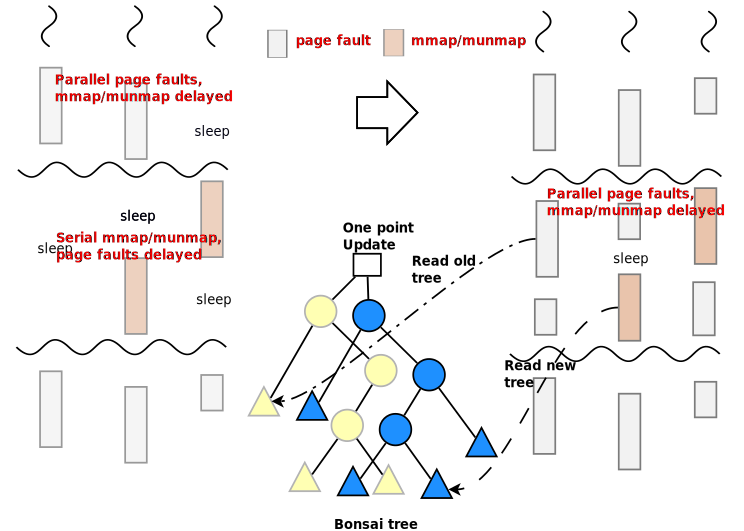
\includegraphics[width=1\textwidth]{fig/bosaivm/bosaivm}
    \caption{Address space 문제와 BosaiVM을 이용한 해결}
  \label{fig:bonsaivm}
\end{figure}

그림~\ref{fig:bonsaivm}의 왼쪽 부분은 이러한 Address Space의 문제를 보여준다. 
병렬로 수행이 가능한 페이지 폴트 때문에 \code{mmap/munmap} 함수에 의해 스레드들은 블락이 걸리고, 병렬로 
수행이 불가능한 \code{mmap/munmap} 함수가 수행되면, \code{mmap/munmap} 함수 뿐만 아니라 
페이지 폴트가 발생한 스레드들까지 블락에 걸린다.
이러한 Single Address Space 문제를 해결하기 위해, 앞에서 설명한 Corey 운영체제와 같이 새로운 운영체제를 
만드는 등 여러 연구들이 진행되었지만, 이 연구에서는 기존 리눅스 커널을 대상으로 구현하였다.
방법은 동기화 기법 중 하나인 RCU와 새로운 밸런스 트리(\code{Bonsai})를 이용하여 Single Address Space 문제를
해결하였다.
즉 리눅스 커널을 대상으로 확장성을 개선한 연구이며, 
리눅스 커널 중 상당히 복잡한 가상 메모리 시스템에 직접 RCU라는 동기화 기법을 적용하여, 
성능 확장성을 향상 시킨 연구이다.
 
BonsaiVM은 총 3가지 기법(\textit{fault locking, hybrid locking/RCU, pure RCU})을 통해
Single Address Space 문제를 해결하였다.
이 중 앞의 두 가지 방법은 리눅스 커널의 구현 의존 적인 해결 방법이고, \textit{pure RCU}는 
기존 리눅스 커널의 레드-블랙 트리를 사용하지 않고 RCU를 사용할 수 있는 
새로운 \code{Bonsai} 트리 자료구조를 만들어 문제를 해결한 방법이다. 
\code{Bonsai} 트리는 그림~\ref{fig:bonsaivm}와 같이 이진 트리로 구성되어 있다. 
\code{Bonsai} 트리의 가장 큰 특징은 루트 노드의 업데이트가 원자적 명령으로 한번에 이루어 진다는 것이다. 
그 이유는 Bonsai 트리는 함수형 트리 형식으로 개발되어서, 밸런스를 수행하는 동안에도 읽기 연산들은 
오래된 트리의 값을 읽을 수 있으며, 병렬로 수행할 수 있는 장점을 가진다는 것이다.
즉 RCU의 장점을 활용하여 여러 읽기 연산과 한가지의 쓰기 연산을 수행하는 스레드들을 병렬로 수행할 수 
있는 장점을 가진다. 
하지만 \code{Bonsai} 트리는 여러 스레들간에 경쟁이 발생하지 않는 경우, 트리 검색이 기존 레드-블랙 트리에 비해 많은 성능 
오버헤드를 가지는 문제점이 있다. 
 
%$$$$$$$$$$$$$$$$$$$$$$$$$$$$$$$$$$$$$$$$$$$$$$$$$$$$$$$$$$$$$$$$$$$$$$$$$$$$$$$$
%Paragraph 2: 기법 설명
%$$$$$$$$$$$$$$$$$$$$$$$$$$$$$$$$$$$$$$$$$$$$$$$$$$$$$$$$$$$$$$$$$$$$$$$$$$$$$$$$

\subsubsection{RadixVM}

%$$$$$$$$$$$$$$$$$$$$$$$$$$$$$$$$$$$$$$$$$$$$$$$$$$$$$$$$$$$$$$$$$$$$$$$$$$$$$$$$
%Paragraph : RadixVM 특징 설명
%$$$$$$$$$$$$$$$$$$$$$$$$$$$$$$$$$$$$$$$$$$$$$$$$$$$$$$$$$$$$$$$$$$$$$$$$$$$$$$$$
RadixVM은 BosaiVM과 같은 연구 그룹이 수행한 연구이며, 
Single Address Space 때문에 발생하는 확장성 문제를 해결하기 위해, 연구 용 운영체제인 sv6의 가상 메모리에 
대한 부분을 수정하여 Single Address Space 문제를 해결한 연구이다.
그 이유는 리눅스의 가상 메모리를 수정하는 것은 굉장히 복잡하여 리눅스 커널에 직접 적용하기에는 힘든 문제점이 
있기 때문에, 상대적으로 덜 복잡한 sv6 운영체제에 새로운 개념인 RadixVM을 적용하였다. 
RadixVM은 BonsaiVM과 같이 가상 메모리 시스템에서 공유되는 Address Space가 \code{mmap, unmap, page
fault} 함수 들로 인해 서로 경쟁함으로 발생하는 문제를 3가지 접근을 통해 해결하였다. 

\begin{figure}[h!]
    \centering
    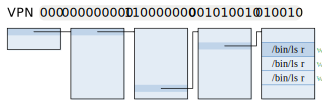
\includegraphics[width=1\textwidth]{fig/radix/radix}
    \caption{RadixVM의 해결 방법}
  \label{fig:radix}
\end{figure}

%$$$$$$$$$$$$$$$$$$$$$$$$$$$$$$$$$$$$$$$$$$$$$$$$$$$$$$$$$$$$$$$$$$$$$$$$$$$$$$$$
%Paragraph : RadixVM  기법 설명 - 1
%$$$$$$$$$$$$$$$$$$$$$$$$$$$$$$$$$$$$$$$$$$$$$$$$$$$$$$$$$$$$$$$$$$$$$$$$$$$$$$$$
첫째, 기존 밸런스 트리를 사용하지 않고, 기수(\code{Radix}) 트리를 이용하는 것이다. 
그 이유는 RadixVM의 궁극적인 목적은 가상 메모리와 관련된 연산에 대해서 최대한 공유를 피하자는 것이다, 
가장 쉬운 방법으로는, 모든 메모리 맵을 배열로서 만들면 모든 가상 메모리 관련 연산들의 충돌은 일어나지 않기 때문에 
쉽게 해결된다.
하지만 단순히 배열을 이용한 방법은 너무 많은 메모리 사용량이 요구된다.
메모리 오버헤드 문제를 해결하기 위한 가장 좋은 방법은 하드웨어 페이지 테이블처럼 동작하는 
기수 트리를 이용하는 것이다.
이처럼 기수 트리는 트리의 읽기와 쓰기 연산을 메모리의 서로 다른 부분에 접근하도록 만들어 준다.
따라서 배열을 사용한 방법과 같이 충돌 없이 사용 가능함과 동시에 메모리 오버헤드도 함께 줄일 수 있다.
결론적으로 여러 스레드들이 접근 할 수 있을 뿐 만아니라 메모리 사용량도 밸런스 트리와 비슷한 
수준을 유지 할 수 있는 장점을 가진다.

%$$$$$$$$$$$$$$$$$$$$$$$$$$$$$$$$$$$$$$$$$$$$$$$$$$$$$$$$$$$$$$$$$$$$$$$$$$$$$$$$
%Paragraph : RadixVM  기법 설명 - 2
%$$$$$$$$$$$$$$$$$$$$$$$$$$$$$$$$$$$$$$$$$$$$$$$$$$$$$$$$$$$$$$$$$$$$$$$$$$$$$$$
\code{RadixVM}의 두번째 기법은 \code{munmap}할 때 발생하는 \textit{TLB shutdown} 문제를 해결 한다.
이러한 \textit{TLB shutdown} 문제가 발생하는 이유는 다음과 같다. 
\code{unmap} 함수는 반드시 어떠한 코어의 페이지도 
매핑이 안된 상태로 끝나야 하는데, 이를 유지하기 위해 \code{unmap}
함수는 모든 코어에 \textit{TLB shutdonw} 메시지를 남긴다.
결국 코어가 증가 할 수록 모든 코어에
\textit{TLB shutdown} 메시지를 발생 시키므로 성능 문제가 발생 된다.
\code{RadixVM}에서는 이러한 \textit{TLB shutdown} 문제를 퍼코어 페이지 테이블을 이용하여 해결하였다. 

%$$$$$$$$$$$$$$$$$$$$$$$$$$$$$$$$$$$$$$$$$$$$$$$$$$$$$$$$$$$$$$$$$$$$$$$$$$$$$$$$
%Paragraph : RadixVM  기법 설명 - 2
%$$$$$$$$$$$$$$$$$$$$$$$$$$$$$$$$$$$$$$$$$$$$$$$$$$$$$$$$$$$$$$$$$$$$$$$$$$$$$$$
\code{RadixVM}의 마지막 기법은 새로운 \code{refcache}라는 레퍼런스 카운터(Reference Counter)이다. 
실제 운영체제에서 레퍼런스 카운터는 가장 큰 확장성 저해요소 중에 하나이다.
그 이유는 레퍼런스 카운터는 많은 캐시 일관성 트래픽을 발생 시키기 때문이다.
이러한 레퍼런스 카운터는 기본적으로 3가지 종류로 개발되고 있다. 
먼저 가장 쉬운 방법인 락을 이용하는 방법이 있다. 
즉 모든 증가/감소 명령의 앞뒤에 락을 호출하는 것이다. 
이것은 락 때문에(락 자체가 전변 변수를 이용) 상당히 많은 캐시-라인 경합이 발생된다. 
다른 방법으로는 원자적 증가/감소 명령을 이용하는 것이다. 
하지만 이러한 방법도 결국 전역 변수 때문에 캐시-라인 경합이 발생한다. 
최근의 방법으로는 파티션닝 기법 중 하나인 퍼코어 카운터를 이용하는 것이다. 
하지만, 단순히 퍼코어 카운터를 이용하는 것은 코어 수에 비례하여 공간에 대한 오버헤드를 가지게 된다.
\code{RadixVM}은 이러한 확장성과 메모리 사용량에 대한 오버헤드를 동시에 줄이기 위해, 
특정 시간(Epoch, 10ms)을 기반으로 퍼코어에 저장된 델타 카운트를 
주기적으로 체크하여 퍼코어에 저장된 카운터의 상태를 보고 전역 카운터에 적용하는 방법을 사용한다.
이 방법은 확장성을 높일 수 있을 뿐만 아니라, 동시에 공간에 대한 오버헤드를 줄인다. 

\subsubsection{Scalable Commutativity Rule}

%$$$$$$$$$$$$$$$$$$$$$$$$$$$$$$$$$$$$$$$$$$$$$$$$$$$$$$$$$$$$$$$$$$$$$$$$$$$$$$$$
%Paragraph : SC rule 특징 및 역사 설명 
%$$$$$$$$$$$$$$$$$$$$$$$$$$$$$$$$$$$$$$$$$$$$$$$$$$$$$$$$$$$$$$$$$$$$$$$$$$$$$$$$
SC Rule(Scalable Commutativity Rule)은 MIT PDOS 연구 그룹에서 운영체제의 확장성 개선을 위해 새로운
관점으로 바라본 연구이다.
기존 연구들은 대부분 운영체제의 병목지점을 추출한 후 발견된 병목지점을 해결하기 위해 새로운 
동기화 기법을 개발하거나 기존 개발된 동기화 기법을 적용하는 방법을 이용했다. 
하지만, 이러한 방법들은 모두 워크로드가 다름에 따라 서로 다른 결과를 가지게 되고, 
또한 문제를 해결하는데도 너무 많은 시간이 소요된다는 문제점을 가지고 있다.
실제 확장성에 대한 문제는, 대부분 설계 단계에서 해결 할 수 있으며, 설계 인터페이스를 확장성 있게 만들면, 
확장성 있는 시스템을 쉽게 만들 수 있다는 것을 주장하였다.
그 이유는 기존 개발되어온 운영체제(예를 들어 리눅스)는 응용프로그램이 커널의 자원을 
확장성 있게 사용하면 확장성에 문제가 해결 되기 때문이다. 
따라서, 확장성 있는 설계가 중요하며, 이를 위해 SC Rule은 리눅스 시스템 콜 연산에 대한 가환성(Commutativity)을 정의하였고, 
그에 대한 이론을 설명하였다.
가환성을 예를 들어 설명하면, 원자적으로 값 X를 변수 A에 추가하고, 
다른 CPU가 원자적으로 같은 변수에 Y라는 값을 추가하였다면, 
두 가지의 명령은 순서가 상관이 없고, 결국에는 X + Y의 값이 변수 A에 저장된다는 것이다.
이러한 수학적인 가환성을 리눅스의 시스템 콜을 대상으로 적용하였으며, 새로운 가환성을 정의 하였다.

%$$$$$$$$$$$$$$$$$$$$$$$$$$$$$$$$$$$$$$$$$$$$$$$$$$$$$$$$$$$$$$$$$$$$$$$$$$$$$$$$
%Paragraph : SC rule 예제 설명 
%$$$$$$$$$$$$$$$$$$$$$$$$$$$$$$$$$$$$$$$$$$$$$$$$$$$$$$$$$$$$$$$$$$$$$$$$$$$$$$$$
저자는 SIM(State-dependent, Interface-based, Monotonic)라고 부르는 새로운
POSIX 운영체제의 가환성(commutativity)에 대해서 정의를 하였다.
또한 POSIX의 오퍼레이션에 대한 가환성을 여러 오퍼레이션을 예로 들며 설명하였다.
\code{open(``a'', O\_CREAT|O\_EXCL)}을 두 개의 코어가 같은 디렉토리에서 수행하면 가환성이 없는데, 
이것을 다른 디렉토리에서 수행하면 가환성을 가진다는 것이다.
저자가 주장하는 SIM 가환성은 시스템 콜 함수들을 구별할 수 있게 만들어주고, 결국 
인터페이스 레벨에서 가환성을 가짐에 따라 확장성 있는 시스템을 가질 수 있다는 것이다.  
또 다른 예로 프로세스를 복사하는 \code{fork()}는 가환성이 없는데, 
\code{fork()}를 \code{posix\_spawn()}으로 수정하면 가환성을 가지게 되고, 이것은 결국 
시스템의 확장성을 향상 시키게 된다. 
이러한 원리는 결국 앞에서 설명하였듯이, 리눅스는 응용프로그램의 방법에 따라 확장성을 가질 수 있다는 것을 
활용한 연구이며, 이 연구는 리눅스 특성들을 잘 이용한 연구이다. 
결국 리눅스 커널은 가환성을 잘 지키도록 호출 해주면, 확장성을 향상 시킬 수 있고 
이것은 설계 단계에서 처리가 가능하다는 것이다. 
또한 저자는 QEMU을 수정하여 리눅스의 가환성을 분석 할 수 있는 \code{Commuter}라는 툴을 제공한다. 
이러한 툴을 통해 설계 단계에서 확장성 문제를 발견할 수 있도록 하였으며, 이 툴을 통해 저자가 
직접 운영체제(리눅스, sv6)의 문제점을 분석하였다. 

%$$$$$$$$$$$$$$$$$$$$$$$$$$$$$$$$$$$$$$$$$$$$$$$$$$$$$$$$$$$$$$$$$$$$$$$$$$$$$$$$
% Paragraph 3: Scalable Data Structure and Lock에 대한 연구
%$$$$$$$$$$$$$$$$$$$$$$$$$$$$$$$$$$$$$$$$$$$$$$$$$$$$$$$$$$$$$$$$$$$$$$$$$$$$$$$$
\newpage
\section{확장성 있는 락 연구}
\label{sec:lockrelated}

%$$$$$$$$$$$$$$$$$$$$$$$$$$$$$$$$$$$$$$$$$$$$$$$$$$$$$$$$$$$$$$$$$$$$$$$$$$$$$$$$
%Paragraph : 기본적인 락에 대한 이야기와 확장성 있는 락의 필요성 
%$$$$$$$$$$$$$$$$$$$$$$$$$$$$$$$$$$$$$$$$$$$$$$$$$$$$$$$$$$$$$$$$$$$$$$$$$$$$$$$$
락은 기본적으로 여러 스레드들을 안전하고, 올바르게 동작하도록 만들어주는 목적을 가진다.
이처럼 여러 스레드를 안전하게 동작 시켜주기 위해, 원자적 명령어인 하드웨어 동기화 명령들(CAS,
fetch-and-add, SWAP 등)을 이용하여 구현되어 왔다. 
즉 코어들과 램(RAM)간에는 공유하는 버스가 있고, 이러한 버스를 원자적으로 
처리하기 위해 하드웨어 동기화 명령을 이용한다. 
예를 들어 x86 시스템 같은 경우 하드웨어 동기화 명령인 \code{xchg} 명령어를 통해 쉽게 락을 구현할 수 있다.
하지만 실제 시스템은 보다 더 복잡한 구조로 되어 있는데, 
실제로 복잡한 이유는 하드웨어에서 고려해야할 사항이 있기 때문이다. 
먼저 중간에 캐시 메모리와 일관성을 유지하기 위한 캐시 일관성 
프로토콜 때문에 발생하는 문제를 고려해야 하고, NUMA 구조이기 때문에 발생하는 여러 문제를 고려해야 한다. 


%$$$$$$$$$$$$$$$$$$$$$$$$$$$$$$$$$$$$$$$$$$$$$$$$$$$$$$$$$$$$$$$$$$$$$$$$$$$$$$$$
%Paragraph : 리눅스 락 구현에 대한 이야기
%$$$$$$$$$$$$$$$$$$$$$$$$$$$$$$$$$$$$$$$$$$$$$$$$$$$$$$$$$$$$$$$$$$$$$$$$$$$$$$$$
전통적으로 락 프리미티브(Primitive)는 두 종류로 구현되어 왔다.
하나는 바쁜대기(Busy-waiting) 방법과 다른 하나는 슬리핑(Sleeping) 또는 블락킹(Blocking) 방법으로 구현된다.
만약 락을 잡고 있는 시간이 적을 때는 바쁜대기(Busy-waiting) 방법을 사용한다. 
이 방법은 락이 풀릴 때까지 전역 변수를 CAS연산을 사용하여 반복 적으로 전역 변수를 읽음으로써 구현된다.
이것은 블락킹 오버헤드(스케줄링 오버헤드) 줄일 수 있으나, 
수행 도중 CPU를 계속 사용함에 따라 다른 스레드들이 CPU를 점유하지 못하게하는 문제를 가진다.
다른 방법인 블락킹 락은 락이 걸려 있는 동안 다른 스레드들을 동작시킬 수 있는 장점을 가지나,
이것은 스케줄러의 스레드 관리에 의존적이고 스케줄링 정책에 따라 공정성등에 영향을 준다.

%$$$$$$$$$$$$$$$$$$$$$$$$$$$$$$$$$$$$$$$$$$$$$$$$$$$$$$$$$$$$$$$$$$$$$$$$$$$$$$$$
%Paragraph : 락과 확장성에 대한 이야기
%$$$$$$$$$$$$$$$$$$$$$$$$$$$$$$$$$$$$$$$$$$$$$$$$$$$$$$$$$$$$$$$$$$$$$$$$$$$$$$$$
최근 운영체제는 이 두 가지 방법을 혼합하여 사용한다. 
즉 리눅스 커널의 블락킹 락은 \code{fastpath, optimistic spinning, slowpath}로 구현된 3가지의
락을 혼합하여 구현된다~\cite{Bueso2014STP}.
예를 들어 커널의 \code{rw\_semaphore}(reader-writer semaphore)는 아래와 같이 3가지 상태로 구현된다.
\begin{itemize}
\item \textbf{fastpath.} 아무도 락을 안잡고 있을 때, 원자적 명령어(\code{fetch\_and\_add})를 이용하여
카운터를 수정하고 락과 함께 반환하는 부분이다.
\item \textbf{optimistic spinning.} 다른 스레드가 락을 잡고 있어서 기다려야 하는 상황이다.
Optimistic Spinning을 수행하는 이유는 대부분 락이 필요한 임계 영역의 크기가 작고, 
이러한 상황에 대해서 블락킹 오버헤드를 줄이기 위해 바쁜대기(busy-waiting)로 수행하는 것이 
효율적이다는 것이다. 
또한 최근에는 모든 코어가 같은 전역 변수를 읽을 경우 많은 캐시 일관성 트래픽이 발생시키므로, 
락을 걸 코어에 등록하고 기다리는 코어에서는 해당 CPU의 로컬 변수만 주기적으로 확인하는 
큐 기반 락(MCS 기반 락)으로 이 부분을 구현한다. 
\item \textbf{slowpath.} 만약 락을 잡고 있는 시간이 길어지면, 대기 큐에 집어 넣고 슬립(Sleep)을 수행하는 블락킹 
락을 수행한다. 
\end{itemize}
이와 같이 하이브리드한 슬리핑 락은 많은 성능 향상을 가진다. 


%$$$$$$$$$$$$$$$$$$$$$$$$$$$$$$$$$$$$$$$$$$$$$$$$$$$$$$$$$$$$$$$$$$$$$$$$$$$$$$$$
%Paragraph :   atomic instructions 이야기
%$$$$$$$$$$$$$$$$$$$$$$$$$$$$$$$$$$$$$$$$$$$$$$$$$$$$$$$$$$$$$$$$$$$$$$$$$$$$$$$$



%$$$$$$$$$$$$$$$$$$$$$$$$$$$$$$$$$$$$$$$$$$$$$$$$$$$$$$$$$$$$$$$$$$$$$$$$$$$$$$$$
%Paragraph :   ts, ticket lock 이야기
%$$$$$$$$$$$$$$$$$$$$$$$$$$$$$$$$$$$$$$$$$$$$$$$$$$$$$$$$$$$$$$$$$$$$$$$$$$$$$$$$


%$$$$$$$$$$$$$$$$$$$$$$$$$$$$$$$$$$$$$$$$$$$$$$$$$$$$$$$$$$$$$$$$$$$$$$$$$$$$$$$$
%Paragraph : 락과 확장성 정리
%$$$$$$$$$$$$$$$$$$$$$$$$$$$$$$$$$$$$$$$$$$$$$$$$$$$$$$$$$$$$$$$$$$$$$$$$$$$$$$$$
확장성을 위해 락과 관련한 병렬 처리에 대하여 고려해야 할 사항들을 정리하면,
기본적으로 락으로 보호해야 할 임계 영역(Critical Region)의 길이를 최대한 짧도록 해야 하고, 
락 자체가 가지고 있는 오버헤드도 또한 고려해야 할 사항이다. 
또한 락의 세분화(Granularity) 정도에 따라 Find-grained 락을 사용할지 Coarse-grained 락을 사용해야 할지 
고려해야 한다.

다음으로, 읽기-쓰기 비율을 고려하여 읽기가 많은 경우에는 읽기-쓰기 락을 사용하고,
읽기가 많으며 오래된(stale) 데이터도 문제가 없는 자료구조에서는 RCU 같은 동기화 기법을 사용해야 한다.  
또한 약간의 공정성(Fairness)을 손해 보더라도 NUMA 기반의 확장성을 높이는 방법도 고려해야 한다.
마지막으로 최근 락에 대해서 중요한 요소로 생각하고 있는 캐시 일관성 때문에 발생하는 
오버헤드 역시 고려해야 한다. 

%~\cite{MellorCrummey1991MCS}~\cite{Magnusson1994QLC},
% ~\cite{Wang2016BeMyGuest}, ~\cite{Scott2013SS}
%~\cite{Bueso2014MCS}~\cite{Bueso2015STP}

%

%~\cite{Hendler2010FC}~\cite{Fatourou2012RCS}~\cite{Delegation2014}

이러한 고려 사항들을 적용하여 확장성 있는 락에 대한 연구는 큐 기반의
락과 계층 적 락 그리고 위임하는 방법(Delegation Techniques)들이 연구되고 있다. 
본 연구의 사전 연구 결과물인 과거 버전의 LDU~\cite{Kyong2016LDU}도 위임하는 방법에 속하며, 
이 방법은 로그를 퍼코어 방법이 아닌 전역 큐에 저장하는 방법을 사용한 연구이다.

\subsection{큐 기반의 락(Queued Lock)}
%\subsubsection{MCS}
%$$$$$$$$$$$$$$$$$$$$$$$$$$$$$$$$$$$$$$$$$$$$$$$$$$$$$$$$$$$$$$$$$$$$$$$$$$$$$$$$
%Paragraph :   MCS 이야기
%$$$$$$$$$$$$$$$$$$$$$$$$$$$$$$$$$$$$$$$$$$$$$$$$$$$$$$$$$$$$$$$$$$$$$$$$$$$$$$$$
모든 코어가 바라보는 전역 변수를 사용하기 때문에 발생하는 캐시 일관성 트래픽 문제는 
락 내부에서도 발생한다. 
그 동안 락의 구현은 하나의 전역변수를 대상으로 원자적 명령을 이용하여 구현되어 왔다.
따라서 자연히 캐시 일관성 트래픽 문제가 발생하였는데, 이것을 해결하는 방법이 큐 기반의 락
~\cite{MellorCrummey1991MCS}~\cite{Magnusson1994QLC}~\cite{Wang2016BeMyGuest}~\cite{Scott2013SS}
~\cite{Bueso2014MCS}을 이용하는 것이다. 

락 때문에 발생하는 캐시 일관성 문제를 해결하기 위한 가장 쉬운 접근하는 방법은 각 
코어가 모두 다른 캐시 라인의 데이터를 가지고 스핀을 하면 된다.
즉 각각의 코어가 \textit{read-only} 스핀을 하고, 반환 하는 스레드가 명시적으로 해당 코어의 캐시 라인의 데이터를 
원자적 명령을 이용하여 락을 반환하는 것이다. 
이러한 방법의 문제점은 공간적인 문제가 있다. 
즉 모든 락이 모든 코어의 중복되지 않도록 공간을 확보해야 한다.
이것은 현실적으로 메모리 낭비가 심히다.
이러한 문제를 해결한 것이 CLH 큐 기반 락이다. 
이것은 배열 기반으로 모든 코어가 같은 전역 변수를 바라 보며 스핀하지 않고, 
각자의 로컬 변수를 바라 보며 스핀하도록 하여, 확장성을 향상 시킨 방법이다. 
즉 기존 많은 공간(락 * 스레드 수)이 필요한 것을 적은 공간(락 + 스레드 수)로도 구현이 가능하도록 한것이다.

또한 배열 기반 방법의 메모리 낭비를 더 줄이기 위해 MCS 락이 개발되었다. 
이러한 MCS 락은 락에 대한 정보를 링크드 리스트로 보관하자는 것이 기본적인 아이디어이고, 
MCS는 하나의 스레드는 반드시 하나의 락만 기다린다는
아이디어를 활용하여 링크드 리스트로 기다리는 스레드들을 관리하였다. 
 
%$$$$$$$$$$$$$$$$$$$$$$$$$$$$$$$$$$$$$$$$$$$$$$$$$$$$$$$$$$$$$$$$$$$$$$$$$$$$$$$$
%Paragraph 2: scalable locks의 성능에 대한 이야
%$$$$$$$$$$$$$$$$$$$$$$$$$$$$$$$$$$$$$$$$$$$$$$$$$$$$$$$$$$$$$$$$$$$$$$$$$$$$$$$$
코어 수가 적을 경우 티켓 락이 더 높은 성능을 보이지만, 
코어 수가 많아 질수록 MCS 락이 좋은 성능을 보인다. 
이처럼 확장성 있는 락을 사용하면, 락 때문에 발생하는 확장성 문제 즉 성능이 갑자기 떨어지는 현상을 
방지할 수 있다.
%하지만 근본적으로 확장성 있는 시스템을 구축하려면 반드시 임계 영역의 길이를 줄여야 한다.
이러한 장점을 받아들여, 리눅스 커널도 처음에는 티켓 락 기반의 스핀락을 사용했으나, 
2013년 이후 티켓-스핀락을 MCS-스픽락으로 변경하였다. 
엄밀하게 말하면 리눅스 커널은 MCS의 기본적인 자료구조 사이즈가 크기 때문에, MCS 락을 커널 크기에 
맞도록 최적화하여 사용한다. 
결국 2016년 부터 리눅스 커널에서 티켓 락 기반의 스핀락은 사라지게 되었다~\cite{ticket}.
 
\subsection{계층적 락}

%$$$$$$$$$$$$$$$$$$$$$$$$$$$$$$$$$$$$$$$$$$$$$$$$$$$$$$$$$$$$$$$$$$$$$$$$$$$$$$$$
%Paragraph 2: 계층적 락
%$$$$$$$$$$$$$$$$$$$$$$$$$$$$$$$$$$$$$$$$$$$$$$$$$$$$$$$$$$$$$$$$$$$$$$$$$$$$$$$$
계층적인 락~\cite{Radovic2003HBL}~\cite{Chabbi2016CLL}~\cite{Luchangco2006HCQ}
~\cite{Chabbi2015HPL}의 공통적인 목적은 스케일이 큰 NUMA 환경에서 확장성을 높이는 것이다.  
NUMA 환경에서는 원격 소켓에 데이터를 접근하는 것 때문에 성능이 저하되는 문제를,
소켓 단위로 락의 이주(Migration)을 줄여서 성능을 향상 시키는 방법이다.
또한 이러한 계층적 락에 대한 연구는 여러 소켓을 전역 락과 소켓 안에서 관리하는
지역 락을 따로 두어 약간의 공정성(Fairness)을 손해 보더라도, 
NUMA 노드의 지역성을 향상 시켜서 성능을 향상 시키는 방법을 사용한다.

\subsection{Delegation techniques}

\subsubsection{Flat Combining}

%$$$$$$$$$$$$$$$$$$$$$$$$$$$$$$$$$$$$$$$$$$$$$$$$$$$$$$$$$$$$$$$$$$$$$$$$$$$$$$$$
%Paragraph :   Flat Combining 이야기
%$$$$$$$$$$$$$$$$$$$$$$$$$$$$$$$$$$$$$$$$$$$$$$$$$$$$$$$$$$$$$$$$$$$$$$$$$$$$$$$$
\code{Flat combining}(FC)~\cite{Hendler2010FC}은 여러 코어에서 캐시 일관성 트래픽 문제를 발생 시키는 
락을 호출하면서 연산을 수행하는 것 보다, 하나의 코어에서 한 스레드가 명령어들을 
모아서 하나의 전역 락을 사용하여 처리하는 것이 더 효율적이라는 것을 이용한 연구이다.
그리고 이러한 철학을 가지고 하나의 동기화 기법으로 만든 것 FC이다.
FC는 두 가지 장점을 가지는데 먼저 FC는 락을 자주 수행하지 않으므로, 락에 의한 
캐시 일관성 트래픽이 상대적으로 덜 발생하고,
하나의 스레드에서 여러 읽기 쓰기 연산을 수행함에 따라, 캐시 지역성이 높아져서 
높은 성능을 가진다는 것이다. 

\begin{figure}[h!]
    \centering
    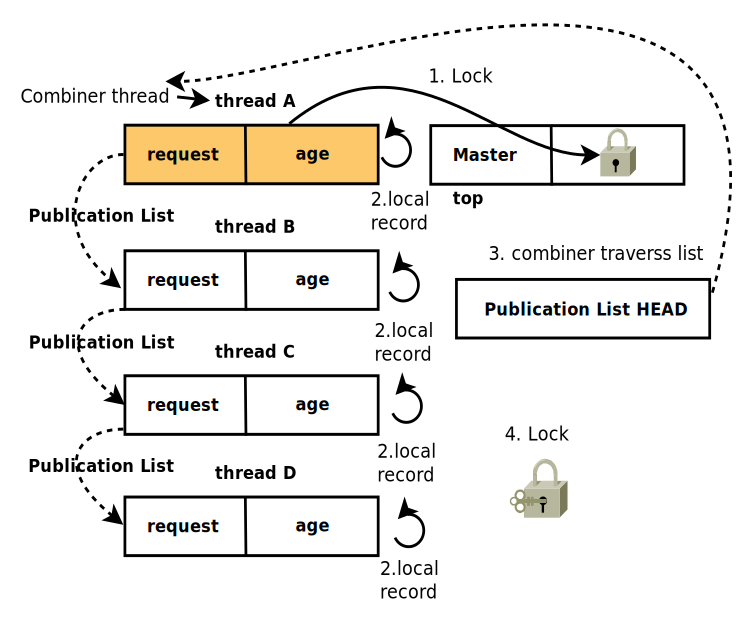
\includegraphics[width=1\textwidth]{fig/FC/FC}
    \caption{Flat Combining 방법}
  \label{fig:FC}
\end{figure}

%$$$$$$$$$$$$$$$$$$$$$$$$$$$$$$$$$$$$$$$$$$$$$$$$$$$$$$$$$$$$$$$$$$$$$$$$$$$$$$$$
%Paragraph :   Flat Combining 알고리즘
%$$$$$$$$$$$$$$$$$$$$$$$$$$$$$$$$$$$$$$$$$$$$$$$$$$$$$$$$$$$$$$$$$$$$$$$$$$$$$$$$
그림~\ref{fig:FC}는 FC 알고리즘의 방법에 대해서 설명한다. 
먼저 자료구조에 대한 연산(예를 들어 스택 같은 경우 \code{push} 또는 \code{pop})이 도착하면, 
처음 받은 스레드는 락을 걸고, 해당 명령어를 수행한다. 
동시에 다른 코어의 스레드들은 다른 명령어들을 수행하게 되는데, 각 코어의 스레드들은 
받은 연산들을 코어의 내부 변수에 요청 정보와 시간 정보(age)를 같이 저장 한다.
처음 받은 스레드의 연산이 끝나면, 이 시점 부터 각 스레드에 저장된 연산들을 순회하면서, 
\code{combiner} 스레드가 모든 연산들을 수행하고, 마지막으로 락을 해제하는 방법으로 수행된다. 

\subsubsection{OpLog}
%$$$$$$$$$$$$$$$$$$$$$$$$$$$$$$$$$$$$$$$$$$$$$$$$$$$$$$$$$$$$$$$$$$$$$$$$$$$$$$$$
%Paragraph 2: OpLog 이야기
%$$$$$$$$$$$$$$$$$$$$$$$$$$$$$$$$$$$$$$$$$$$$$$$$$$$$$$$$$$$$$$$$$$$$$$$$$$$$$$$$

\begin{figure}[h]
    \centering
    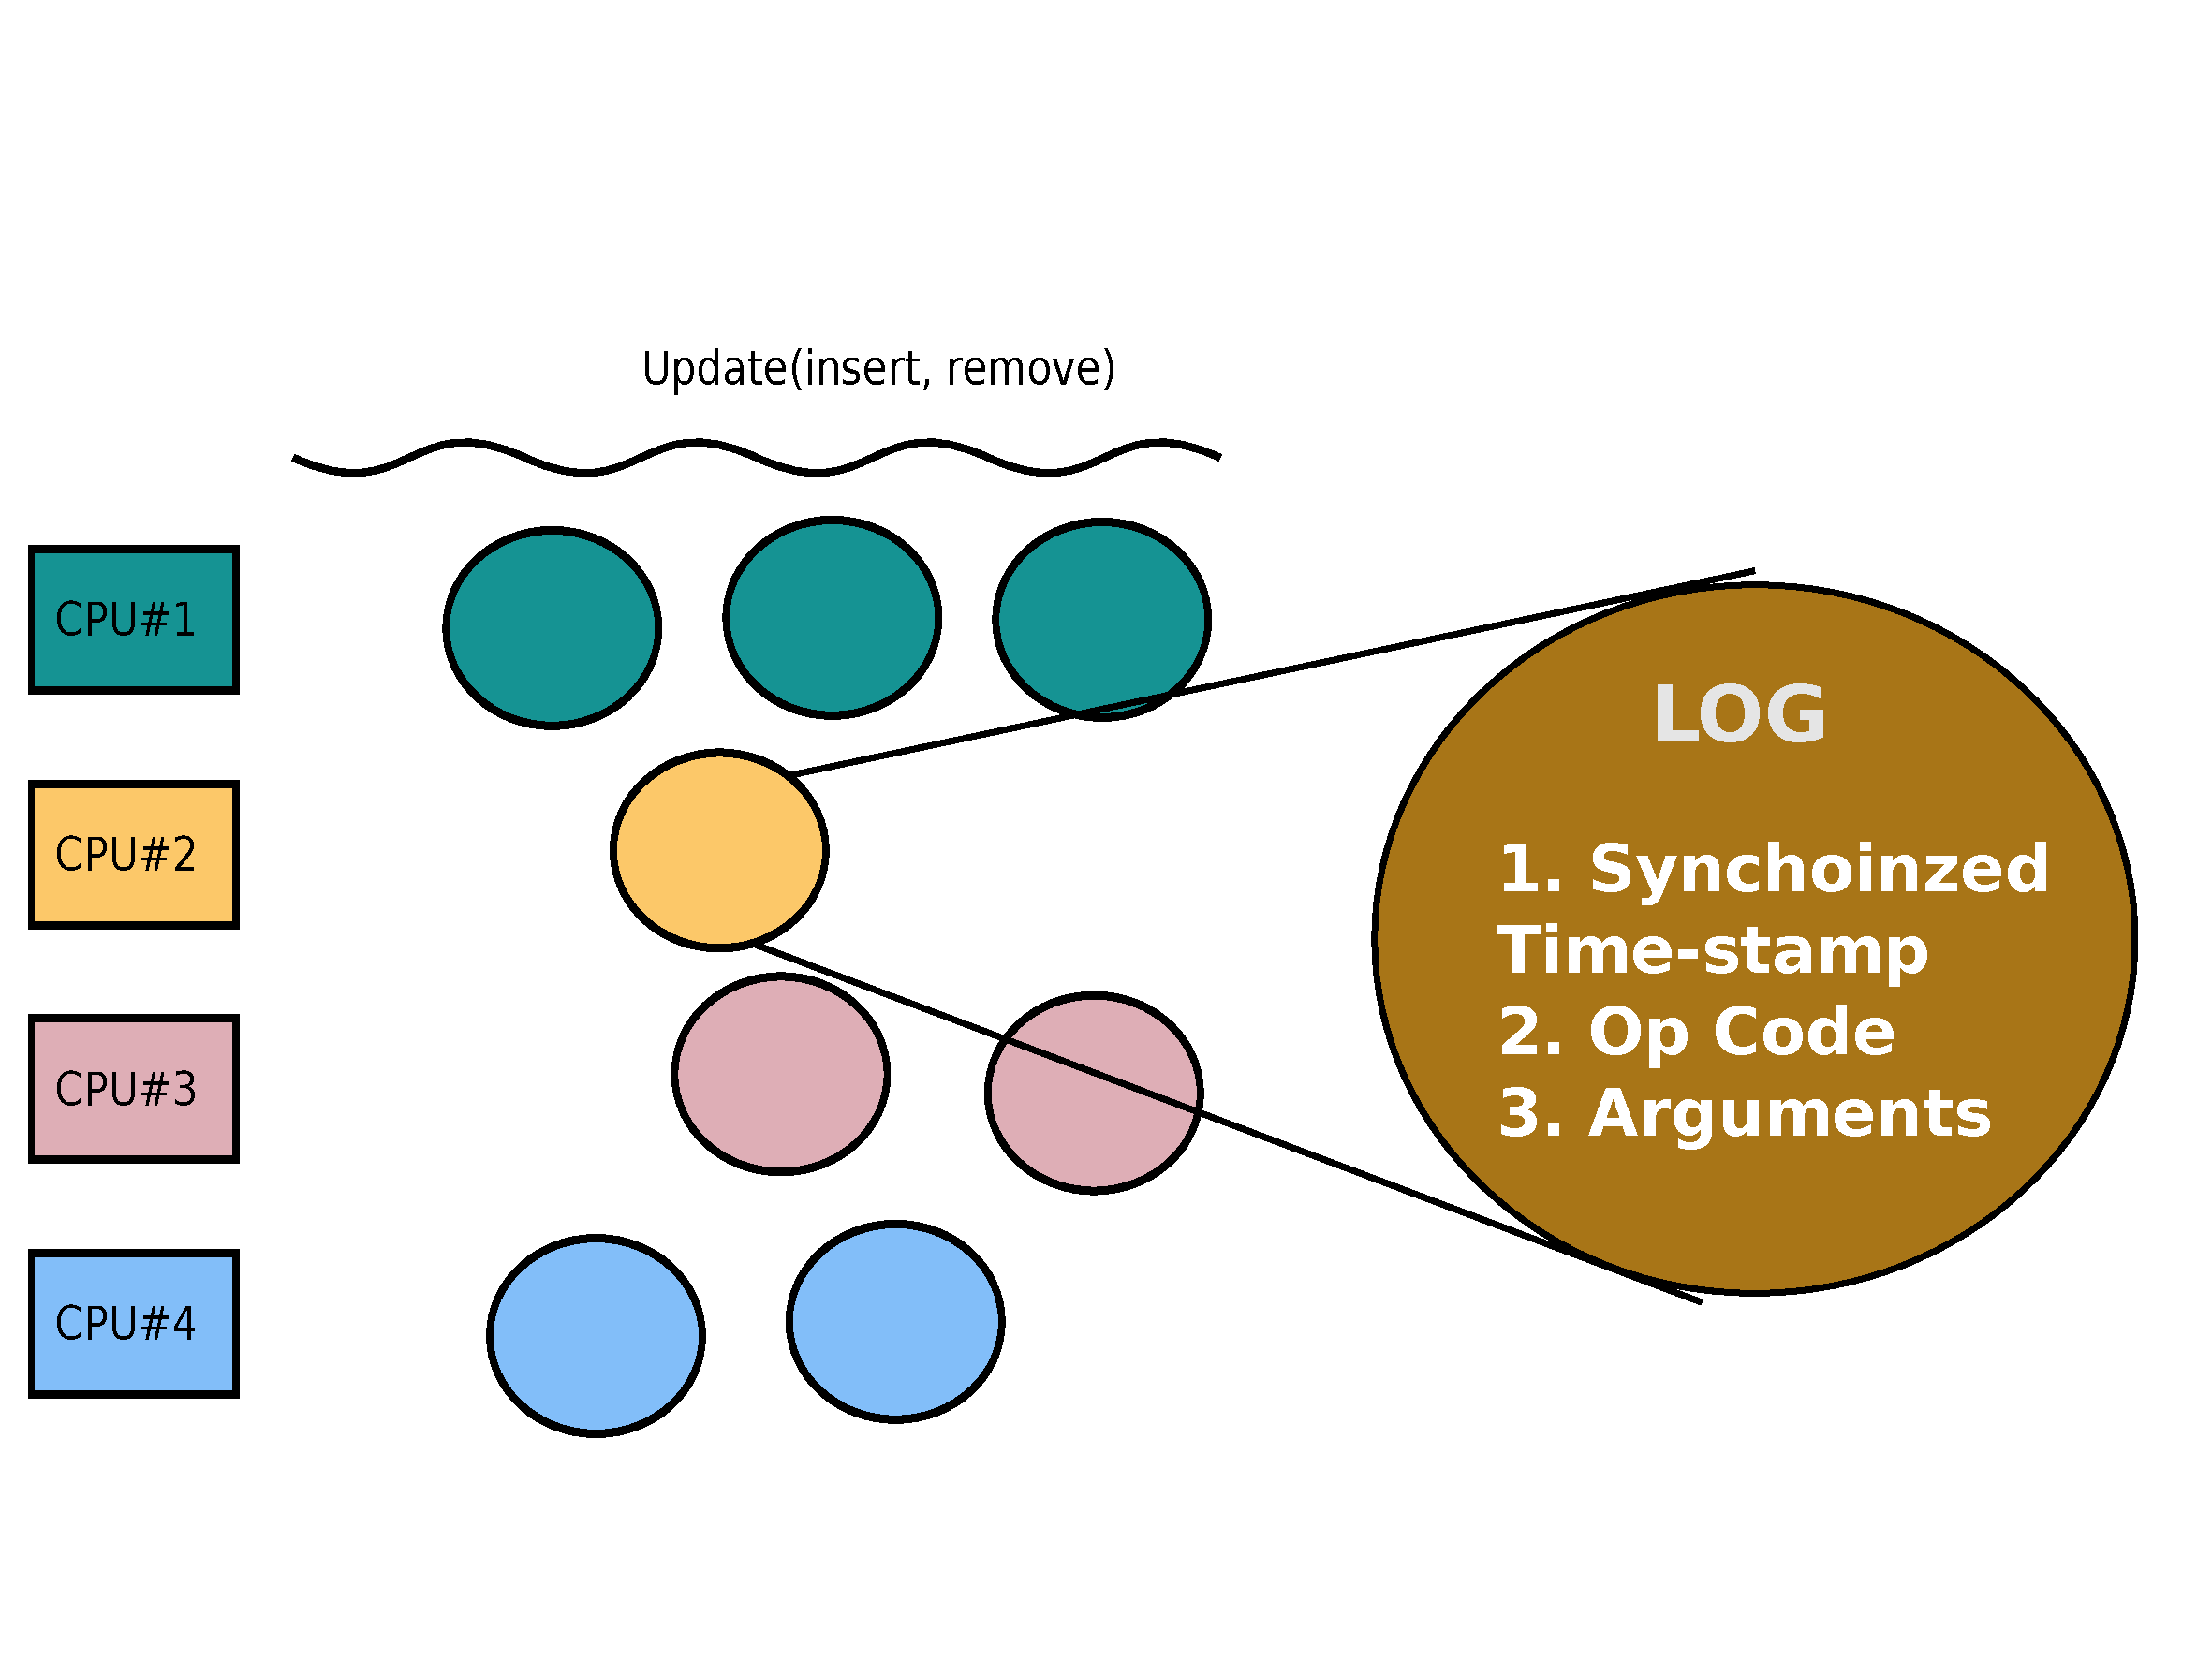
\includegraphics[width=0.8\textwidth]{fig/oplog_log}
    \caption{OpLog의 업데이트 방법}
  \label{fig:oplog}
\end{figure}

OpLog는 RCU와 반대로 업데이트 비율이 높은 \code{Update-heavy}한 자료구조를 위해 만든 
동기화 기법 중 하나이다.
업데이트가 많아질 경우, 락에 의해 문제가 생기는데, 기존 연구들의 해결 방법들은 
CAS등 하드웨어 동기화 명령을 사용하여 공유 데이터를 접근하는 방법을 사용한다.
따라서 이때 발생하는 캐시 일관성 트래픽에 의해 
성능에 문제가 생긴다는 것이다. 
이러한 문제점을 해결하기 위한 방법 중 하나가 로그 기반으로 처리하는 것인데, OpLog는 이러한 로그 기반 
방법을 동기화된 타임 스탬프 카운터를 이용하여 퍼코어에 로그를 저장함으로써 해결하였다. 
각 코어에 동기화된 타임 스탬프와 함께 명령어를 로그로 저장을 한 다음, 읽기 연산이 수행되기 전에 
퍼코어에 저장된 로그를 타임 스탬프 정보 함께 시간 순서대로 처리하는 방법이다.
그림~\ref{fig:oplog}는 각 코어에 저장된 로그 정보를 보여준다.
업데이트 연산이 발생하면, 각 코어는 타임 스탬프 정보, 연산 코드 그리고 연산을 처리하기 위한 
인자 값들을 함께 저장한다.

%$$$$$$$$$$$$$$$$$$$$$$$$$$$$$$$$$$$$$$$$$$$$$$$$$$$$$$$$$$$$$$$$$$$$$$$$$$$$$$$$
%Paragraph 2: OpLog의 타임 스탬프
%$$$$$$$$$$$$$$$$$$$$$$$$$$$$$$$$$$$$$$$$$$$$$$$$$$$$$$$$$$$$$$$$$$$$$$$$$$$$$$$$
이처럼 OpLog는 동기화된 타임스탬프를 이용한다. 
하지만 여러 소켓으로 구성된 NUMA 시스템 같은 경우 소켓별로 \textit{Clock Source}가 다르므로, 
연산 순서가 바뀔 수 있다..
OpLog는 이러한 문제를 동기화 타임스태프 카운터가 있다는 것을 가정하여, 
임시로 소프트웨어 동기화된 타임스탬프 카운터를 구현하여 사용하였다. 
하지만 OpLog는 최근까지 하드웨어적인 동기화 타임스탬프 카운터가 지원하지 않으므로 
현실적으로 적용되는데는 문제가 있다.

%$$$$$$$$$$$$$$$$$$$$$$$$$$$$$$$$$$$$$$$$$$$$$$$$$$$$$$$$$$$$$$$$$$$$$$$$$$$$$$$$
%Paragraph 2:Concurrent updates에 대한 연구
%$$$$$$$$$$$$$$$$$$$$$$$$$$$$$$$$$$$$$$$$$$$$$$$$$$$$$$$$$$$$$$$$$$$$$$$$$$$$$$$$
\newpage
\section{확장성 있는 자료구조 연구}
\label{sec:datarelated}
많은 확장성 있는 방법과 이를 이용하는 자료구조들은 업데이트 비율에 따라 서로 다른 성능을 가진다.
연구자들은 낮거나 중간 정도의 업데이트 비율에서는 새로운 확장성있는
기법~\cite{McKenney98}~\cite{Matveev2015RLU}~\cite{Harris2001Lockfree} ~\cite{Fomitchev2004Lockfree}
~\cite{Timnat2012}을 연구하거나 그 기법을 새로운 자료구조에 
적용~\cite{Arbel2014ConcurrentRCU}~\cite{Dodds2015SCT}~\cite{AustinTClements2012RCUBalancedTrees}을
하도록 시도하고 있다.

\subsection{확장성 있는 자료구조를 위한 동기화 기법}

\subsubsection{RCU}
확장성을 위한 대표적 동기화 기법인 RCU는 McKenney와 Slingwine에 의해 개발되었고, 
이 방법은 동기화 기법 때문에 발생하는 오버헤드를 최소화 시킨 방법이다.
특히 RCU는 리더들을 보호하기 위해 사용하는 동기화 기법에 대한 오버헤드를 최소화 시킨다.
오버헤드가 최소화 되는 이유는 동기화 기법이 캐시 일관성 트래픽 문제를 발생 시키는 전역 변수를 수정하지 않고, 
파티션된 퍼코어 메모리에 상태를 저장하는 방법을 사용하기 때문이다.
따라서 리더들이 수행하는 락의 오버헤드가 적고, 여러 리더 스레드와
하나의 라이터 스레드가 병렬로 수행이 가능하므로 굉장히 높은 확장성을 가질 수 있다.
이러한 장점 때문에 RCU는 현재 리눅스 커널에서 가장 많이 사용되고 있는 동기화 기법 중 하나이다. 
RCU의 단점으로는 RCU의 리더에 비해 라이터가 수행하는 방법은 복잡하므로 라이터가 많아 질 경우 
성능이 저하되는 문제가 있다. 

\begin{figure}[h]
    \centering
    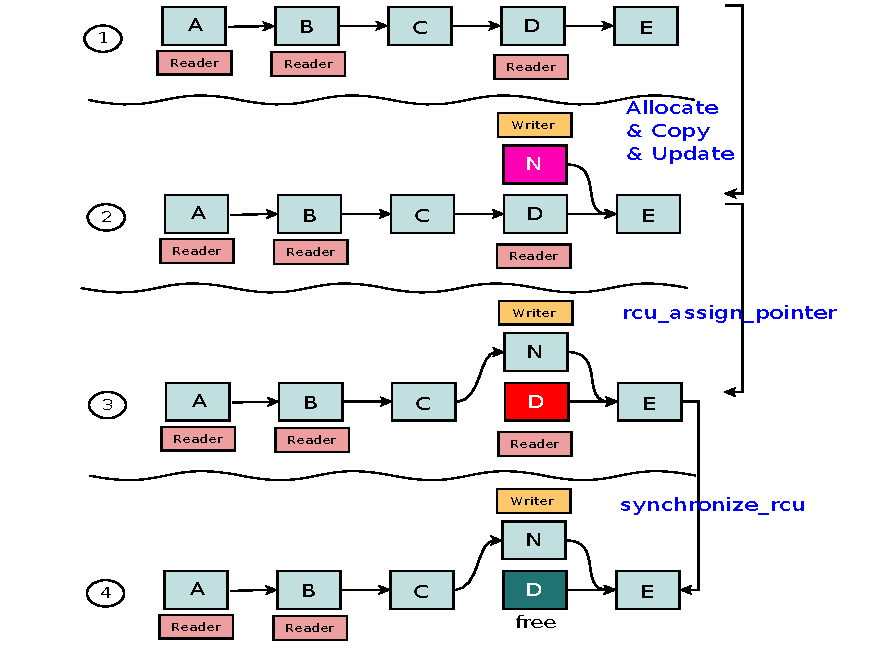
\includegraphics[width=1\textwidth]{fig/rcu/rcu_principle}
    \caption{RCU 예제}
  \label{fig:rcuprinciple}
\end{figure}

%$$$$$$$$$$$$$$$$$$$$$$$$$$$$$$$$$$$$$$$$$$$$$$$$$$$$$$$$$$$$$$$$$$$$$$$$$$$$$$$$
%Paragraph : RCU의 기본 철학
%$$$$$$$$$$$$$$$$$$$$$$$$$$$$$$$$$$$$$$$$$$$$$$$$$$$$$$$$$$$$$$$$$$$$$$$$$$$$$$$$
RCU의 기본 철학은 특정 시점에서 오브젝트를 복제해서 처리하는 것이다. 
그림~\ref{fig:rcuprinciple}은 이러한 RCU의 예를 보여준다.
먼저 그림에서 1단계에는 \code{A, B, C, D, E} 오브젝트 중 \code{A, B, D} 오브젝트를 스레드로 구성된 
리더들이 읽는 모습을 보여준다.
만약 이 순간 \code{D} 오브젝트를 수정하려 하면, RCU는 복사본을 하나 할당 받고, 새로운 오브젝트인 \code{N}을 할당 
받는다.
그리고 다음 단계에서는 원자적인 연산을 통해서 오브젝트 \code{C}와 \code{N}을 연결한다. 
이 순간 오브젝트 \code{D}를 읽고 있는 리더와 다른 리더들은 서로 블락 없이 계속 읽기를 수행할 수 있으며, 
병행으로 업데이트 연산까지 수행할 수 있어서 성능 및 확장성이 향상된다.
마지막 단계로는 \code{synchroinze\_rcu()} 함수를 통해 리더가 읽기 연산를 종료할 때 까지 기다리고, 읽기 연산이
끝나면 바로 \code{free()}를 호출해준다. 
이 때 마지막 리더가 읽을 때 까지 기다리는 시간을 RCU에서는 \textit{grace period}라 부른다.

%$$$$$$$$$$$$$$$$$$$$$$$$$$$$$$$$$$$$$$$$$$$$$$$$$$$$$$$$$$$$$$$$$$$$$$$$$$$$$$$$
%Paragraph : RCU는 기본적으로 3가지 특징
%$$$$$$$$$$$$$$$$$$$$$$$$$$$$$$$$$$$$$$$$$$$$$$$$$$$$$$$$$$$$$$$$$$$$$$$$$$$$$$$$
이러한 RCU는 기본적으로 3가지 특징을 가진다. 
첫 번째로 리더는 락이 필요없다.
실제로 RCU의 리더들은 아무런 락 또는 배리어(Barrier)를 소유하지 않고 수행되며, 읽는 연산에서는 
퍼코어 메모리에 단순히 \textit{enter/exit}를 기록하여 아무런 캐시 일관성 트래픽을 발생 시키지 않으며 수행된다.
두 번째로, 싱글 포인터 업데이트이다.
RCU의 라이터는 원자적 명령으로 싱글 포인터 업데이트를 수행한다.
이러한 특징으로 인해 여러 리더들과 한 가지 업데이트가 동시에 동작할 수 있다.  
마지막으로, RCU는 \code{delayed free}를 수행한다.
즉 노드를 바로 \code{free}를 하지 않고, 모든 리더들이 리드 구역을 벗어난 경우 까지 기다린 후 
해당 노드를 \code{free}한다.
이를 통해 안전하게 자원 해제할 수 있는 특징을 가진다.

\begin{figure}[h]
    \centering
    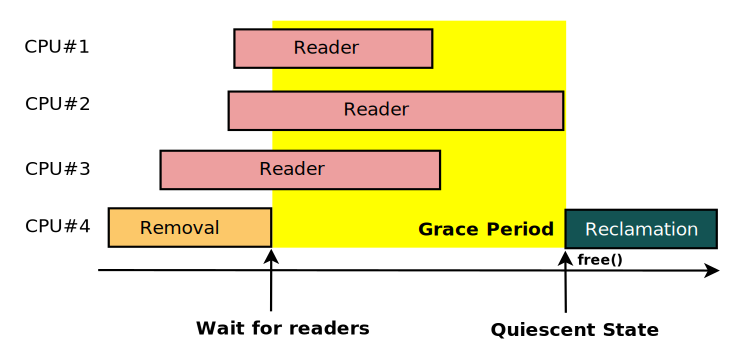
\includegraphics[width=1\textwidth]{fig/rcu/rcu_grace}
    \caption{RCU의 delayed free의 시점}
  \label{fig:rcu_grace}
\end{figure}

%$$$$$$$$$$$$$$$$$$$$$$$$$$$$$$$$$$$$$$$$$$$$$$$$$$$$$$$$$$$$$$$$$$$$$$$$$$$$$$$$
%Paragraph 2: RCU의 grace periad
%$$$$$$$$$$$$$$$$$$$$$$$$$$$$$$$$$$$$$$$$$$$$$$$$$$$$$$$$$$$$$$$$$$$$$$$$$$$$$$$$
그림~\ref{fig:rcu_grace}는 RCU의 \code{delayed free}의 시점을 보여준다.
그림에서 \code{Removal} 명령이 도착하면  RCU는 \code{Removal} 명령을 수행하고 기다린다.  
그 이유는 그 동안 해당 데이터는 리더들이 사용하고 있을 가능성이 있기 때문이다.
그 시점 부터 \textit{grace period} 라고 부르는 리더들이 종료되기를 기다리고, \textit{quiescent
state}라고 부르는 예전 데이터를 읽고 있는 리더들이 없는 상태가 되면 그 때 \code{free()}를 수행한다. 
아직 RCU는 리눅스 스케줄러에 의존하여 \textit{quiescent state}를 판단하나, 
이것은 \textit{grace period}가 길어 질 수 있어 문제가 있다. 
최근에는 이러한 문제를 해결하기 위해 \textit{quiescent state}를 마지막 리더가 끝나는 순간 바로 판단할 
수 있는 방법~\cite{Arbel2015PRR}이 연구되고 있다.

\subsubsection{RLU}

%$$$$$$$$$$$$$$$$$$$$$$$$$$$$$$$$$$$$$$$$$$$$$$$$$$$$$$$$$$$$$$$$$$$$$$$$$$$$$$$$
%Paragraph : RLU가 해결하고자 하는 문제
%$$$$$$$$$$$$$$$$$$$$$$$$$$$$$$$$$$$$$$$$$$$$$$$$$$$$$$$$$$$$$$$$$$$$$$$$$$$$$$$$
RLU는 Alexander Matveev \textit{et al.}이 RCU의 문제점을 해결한 연구이다. 
RCU는 Read-mostly 자료구조에 적합한 방법이나, RCU를 사용하기에는 프로그래머의 상당한 노력이 
필요하고, 라이터들이 증가할 수 록 많은 오버헤드를 가지는 단점이 있다.
또한 RCU의 \code{delayed free}는 모든 리더가 종료했을 때 바로 \code{quiescent state}를 찾는 것이 아니기
때문에 시간에 민감한 응용프로그램에 문제를 가진다. 
이러한 문제를 해결하기 위해 만든 것이 RLU~\cite{Matveev2015RLU}이다. 
RLU는 업데이트 문제를 해결한 로그 기반 알고리즘이나, 
이것은 Read-mostly 자료구조에서 라이터의 원자적 명령어에 의한 오버헤드가 심한 문제를 
싱글 원자적 연산을 사용한 Global Clock 변수와 오브젝트 레벨 안에 퍼코어 단위로 로깅을 사용한 방법을 사용한다.
따라서 업데이트가 많아지면 여전히 확장성 문제가 발생한다. 

\subsubsection{Non-locking 동기화}

%$$$$$$$$$$$$$$$$$$$$$$$$$$$$$$$$$$$$$$$$$$$$$$$$$$$$$$$$$$$$$$$$$$$$$$$$$$$$$$$$
%Paragraph : Non-locking synchronization의 장점
%$$$$$$$$$$$$$$$$$$$$$$$$$$$$$$$$$$$$$$$$$$$$$$$$$$$$$$$$$$$$$$$$$$$$$$$$$$$$$$$$
논블락킹 동기화 방법의 장점은 여러 스레드들이 락 기반으로 자원을 관리함에 따라 
발생하는 여러 문제를 해결할 수 있다.
가장 큰 장점은 스레드 또는 프로세스가 락 때문에 기다리는 시간을 제거할 수 있다.
이 것은 락을 얻기 위해 기다리는 시간을 최소화 할 뿐만 아니라 무한 루프 때문에 무한정 기다리는 
데드락(deadlock) 같은 상황까지 제거 할 수 있다. 
다음으로 앞에서 설명하였듯이 코어 수가 증가 할 수록 락 자체를 얻기 위해 원자적 명령을 이용하는데 이것은 
캐시 일관성 트래픽을 발생한다. 
논블락킹 방법들은 이러한 락 오버헤드를 제거할 수 있다. 
이와 같이 논블락킹 방법은 락 자체가 가지고 있는 문제점인 데드락, 라이브락(Livelock), 
우선순위 역전 현상(Priority Inversion)등을 한번에 제거 할 수 있다. 
또한 논블락킹 동기화 기법을 사용하는 \code{lock-free} 자료 구조들은 성능을 향상 시킬 수 있는데, 
그 이유는 멀티코어 환경에서 공유되는 데이터를 접근하기 위해 여러 스레드가 마치 바쁜대기 처럼 동작하므로 
직렬화 되는 부분이 매우 짧다.

\begin{figure}[h!]
    \centering
    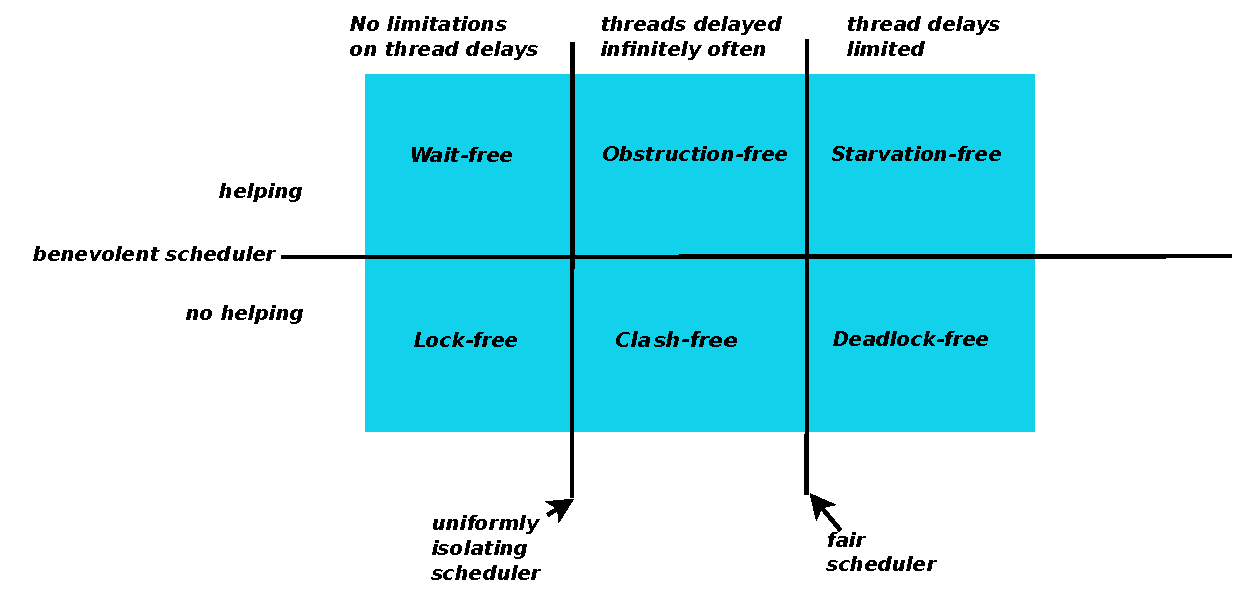
\includegraphics[width=1\textwidth]{fig/NBS/NBS}
    \caption{Non-locking 동기화 기법의 분류}
  \label{fig:NBS}
\end{figure}


%$$$$$$$$$$$$$$$$$$$$$$$$$$$$$$$$$$$$$$$$$$$$$$$$$$$$$$$$$$$$$$$$$$$$$$$$$$$$$$$$
%Paragraph : Non-locking synchronization 알고리즘 종류 1 
%$$$$$$$$$$$$$$$$$$$$$$$$$$$$$$$$$$$$$$$$$$$$$$$$$$$$$$$$$$$$$$$$$$$$$$$$$$$$$$$$
이러한 논블락킹 동기화 기법은 그림~\ref{fig:NBS}와 같이 분류된다.
크게 보면 \textit{Wait-free}방법과 \textit{Wait-free}으로 구분되고, 이것은 1990대 초에 구분되었다.  
\textit{Wait-free} 방법은 가장 구현하기 힘든 알고리즘이며, 모든 스레드가 딜레이 없이 바로 종료할 수 
있는 알고리즘이다. 
다음으로 \textit{Lock-free} 방법은 적어도 하나의 스레드는 딜레이 없이 바로 끝나는 방법이다. 
즉 그 이외의 스레드들은 전역 변수를 동시에 접근해서 발생하는 충돌 때문에 다시 순회할 가능성이 있는 
알고리즘이다.

\begin{figure}[h!]
\begin{center}
\inputminted[linenos,fontsize=\footnotesize,
tabsize=4]{c}{src/lockfree_stack.c}
\end{center}
\caption{간단한 Non-blocking 스택 알고리즘.}
\label{fig:nonblockingstack}
\end{figure}


%$$$$$$$$$$$$$$$$$$$$$$$$$$$$$$$$$$$$$$$$$$$$$$$$$$$$$$$$$$$$$$$$$$$$$$$$$$$$$$$$
%Paragraph : 심플 스택 알고리즘 설명
%$$$$$$$$$$$$$$$$$$$$$$$$$$$$$$$$$$$$$$$$$$$$$$$$$$$$$$$$$$$$$$$$$$$$$$$$$$$$$$$$
이러한 장점을 가진 논블락킹 알고리즘의 스택의 예는 그림 \ref{fig:nonblockingstack}과 같이
구현되어 있다.
자료구조(\code{struct element})의 내용은 \code{value}와 다음 노드를 가리키는 포인터(Line 4)가 존재한다.
\code{push} 함수 같은 경우를 보면, 먼저 새로운 노드의 스택의 \code{top}에 해당하는 노드를 저장(Line 12)하고, 
CAS 연산을 통해 원자적으로 수정되었는지 체크를 함과 동시에 스택의 top에 해당하는 노드를 새로운 노드로 수정한다.
만약 CAS 연산이 실패하였다면(Line 13) 이 경우는 다른 스레드가 수정하였다는 것을 의미한다.
따라서 다시 처음 작업으로 이동(Line 11) 후 앞에서 수행한 일을 반복하여 수행한다.
\code{pop} 함수는 먼저 스택의 \code{top}에 해당하는 포인터를 지역 변수에 저장 후(Line 20), CAS 연산을 통해 
원자적으로 top 다음 포인터를 가르키게 한 후(Line 21) top에 해당하는 노드를 반환한다(Line 23). 
만약 CAS 연산이 실패하면 \code{push} 처럼 처음 부터 같은 일을 반복 수행한다(Line 19).

%$$$$$$$$$$$$$$$$$$$$$$$$$$$$$$$$$$$$$$$$$$$$$$$$$$$$$$$$$$$$$$$$$$$$$$$$$$$$$$$$
%Paragraph : ABA 문제 설명
%$$$$$$$$$$$$$$$$$$$$$$$$$$$$$$$$$$$$$$$$$$$$$$$$$$$$$$$$$$$$$$$$$$$$$$$$$$$$$$$$
논블락킹 동기화 기법의 가장 큰 현실적인 문제점은 바로 중간에 값은 같으나 노드의 메모리 주소가 
바뀔 수 있다는 것이다. 
예를 들어 스택에 \code{top->A->B->C}세가지 노드가 순차적으로 들어 있을 경우, 
CPU\#1이 A를 꺼내고자 top의 포인터를 B를 가리키기 위해서 \code{CAS(top, A, B)} 연산을 
수행하기 전에 바로 선점 되어,  
CPU\#2가 A와 B를 꺼내고 A, B를 \code{free}한 후 다시 새로운 값과 함께 전에 사용한 A 주소를 재 사용하고 
스택에 넣으면, 결국 CPU\#1의 \code{CAS(top, A, B)} 명령어는 성공하게 된다.
따라서 원하는 스택의 결과는 \code{top->C}을 얻어야 하는데, 그렇지 않고 \code{top->B->C} 순서로 스택에 쌓이게
된다.
이러한 상황을 ABA 문제라고 한다. 
이러한 문제의 간단한 해결책은 \code{free()}를 바로 호출하지 않고, 레퍼런스 카운트를 보고 해제하거나, 
안전한 시간(모든 프로세서가 작업이 끝날 때)까지 기다린 후 호출하는 방법이 있다. 

\subsection{확장성 있는 자료구조}

\subsubsection{Harris Linked List}

%$$$$$$$$$$$$$$$$$$$$$$$$$$$$$$$$$$$$$$$$$$$$$$$$$$$$$$$$$$$$$$$$$$$$$$$$$$$$$$$$
%Paragraph 2: harris 알고리즘 설명
%$$$$$$$$$$$$$$$$$$$$$$$$$$$$$$$$$$$$$$$$$$$$$$$$$$$$$$$$$$$$$$$$$$$$$$$$$$$$$$$$
논블락킹 알고리즘 중 대표적인 알고리즘 중 하나는 2001년도에 발표된 Harris Linked
List~\cite{Harris2001Lockfree}이다.
Harris 알고리즘은 CAS를 이용한 대표적인 알고리즘 중 하나이며, 순서대로 정렬된 노드들을 순회하면서 해당 
노드의 위치의 오른쪽 노드를 찾은 후 CAS로 해당 오른쪽 노드 앞에 새로운 노드를 삽입하는 방법을 사용한다. 

\begin{figure}[h!]
    \centering
    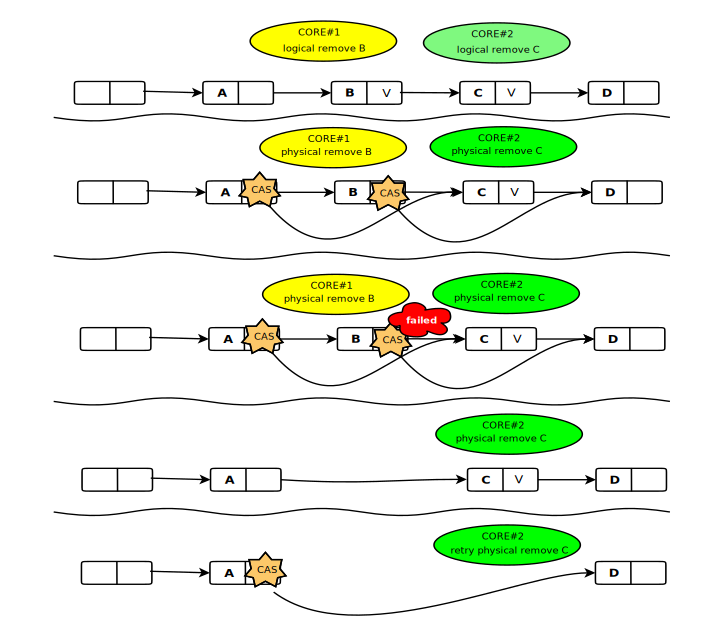
\includegraphics[width=1\textwidth]{fig/harris/harris}
    \caption{Harris 삭제}
  \label{fig:harris}
\end{figure}


%$$$$$$$$$$$$$$$$$$$$$$$$$$$$$$$$$$$$$$$$$$$$$$$$$$$$$$$$$$$$$$$$$$$$$$$$$$$$$$$$
%Paragraph 2: 그림 설명
%$$$$$$$$$$$$$$$$$$$$$$$$$$$$$$$$$$$$$$$$$$$$$$$$$$$$$$$$$$$$$$$$$$$$$$$$$$$$$$$$
이러한 Hariis 알고리즘의 한 예로 삭제 연산에 대해서 설명하면 그림~\ref{fig:harris}과 같다. 
시간 순서 대로 위에서 아래로 진행된다.
동시에 \code{CORE\#1}이 노드 B를 삭제하고 \code{CORE\#2}가 노드 C를 삭제한다면,
Harris 링크드 리스트에서는 삭제를 바로 수행하지 않고 먼저 각 노드에 마킹을 한다. 
Harris 링크드 리스트 알고리즘에서는 이것을 \code{logical remove}라고 한다.
다음으로 \code{CORE\#1}과 \code{CORE\#2}가 동시에 CAS 연산으로 삭제를 하면, \code{CORE\#2}의 오래된 값이 
\code{CORE\#1}에 의해 변경되었기 때문에 이 순간 CAS 실패가 발생하다. 
CAS 실패에 의해 아직 노드가 남아 있는 상태가 되며, 이미 \code{logical remove}에 의해 
논리적으로 제거된 상태를 남게 된다.  
Harris 리스트는 CAS가 실패하면 처음 부터 다시 순회함과 동시에 마킹된 노드를 다시 CAS 연산을 사용해 
제거한다.
Harris 리스트의 오버헤드는 CAS 연산과 \code{logical remove}에 따른 전역 변수의 수정과 
수정된 노드들을 각 코어들이 CAS 실패 할 때 마다 다시 순회하므로 캐시 일관성 트래픽이 
많이 발생하여 성능에 문제가 있다.

%\subsubsection{Time-stamp stack}



%\newpage
\section{하드웨어}
\label{sec:hwrelated}

\subsection{캐시 일관성(Cache Coherency)}



병렬화를 위한 캐시는\ldots 




\subsection{원자적 명령(Atomic Operations)}

원자적 명령은\ldots



\subsection{메모리 배리어(Memory Barriers)}

메모리 배리어는\ldots








